\documentclass[10pt]{report}
\usepackage{green_buddhism}
\title{Green Buddhism: A Programmer's Religion}
%\subtitle{Enjoying a life of liberty}
\author{Logan Streondj \\
  \doclicenseName}
\begin{document}
\maketitle
\documentclass{report}
\usepackage{green_buddhism}
\begin{document}
\chapter{Introduction}
Here you will learn, the secrets of the cosmos, 
and how you can help us (Earthlings) achieve domain over the solar system, galaxy and
beyond.  

Later this will be a book, but for now here are some basics. 

\subsection{Disclaimer} 
If these secrets are in conflict with your ideology,
then please see this as an imaginary story. 

\end{document}

\section{recent reform}
\begin{itemize}
  \item added English Pirate (\ref{reincarnation:pirate}) 2017/10/09
  \item added War Widow (\ref{reincarnation:widow}) 2016/10/07
  \item added Mammoth Hunter (\ref{reincarnation:mammoth}) 2016/10/04
  \item added Climbing the Reincarnation Stairs (\ref{chapter:climbing})
2016/10/04
  \item added my one muslim reincarnation (\ref{reincarnation:muslim})
2016/10/04
  \item added began itinerary to awakening part (\ref{awakening}) 2016/10/03
  \item added a Logan reincarnation entry about the pagan castle
(\ref{reincarnation:arwald}) 2016/10/03
  \item added Electronic Bodies section (\ref{history:electronic}) 2016/09/30
  \item added Terms of Peaceful Trade Relations section (\ref{terms}) 2016/09/30
  \item added Living in Peace Chapter (\ref{peace}) 2016/09/29
  \item added What is the story of Green Buddhism? (\ref{whatstory}) 2016/09/29
  \item added grey population distribution subsection (\ref{popdist})
2016/10/28
 \item updated Arecibo section (\ref{arecibo}) 2016/09/28
 \item added bibilography (\ref{bibliography}) 2016/09/28
\end{itemize}
\tableofcontents

\chapter{What is the story of Green Buddhism?}
\epigraph{If scientific analysis were conclusively to demonstrate certain claims
in Buddhism to be false, then we must accept the findings of science and abandon
those claims.}
{Dalai Lama XIV\cite{singleAtom}}
\label{whatstory}
In 2009 I went to Thailand to be a monk for a month. I liked the robes but they
said I couldn't wear them when I got back to Canada, unless I was a monk at one
of their temples. However when I asked if I could remake them into a different 
colour, like green or purple and then wear them, they said sure. 

\begin{figure}
  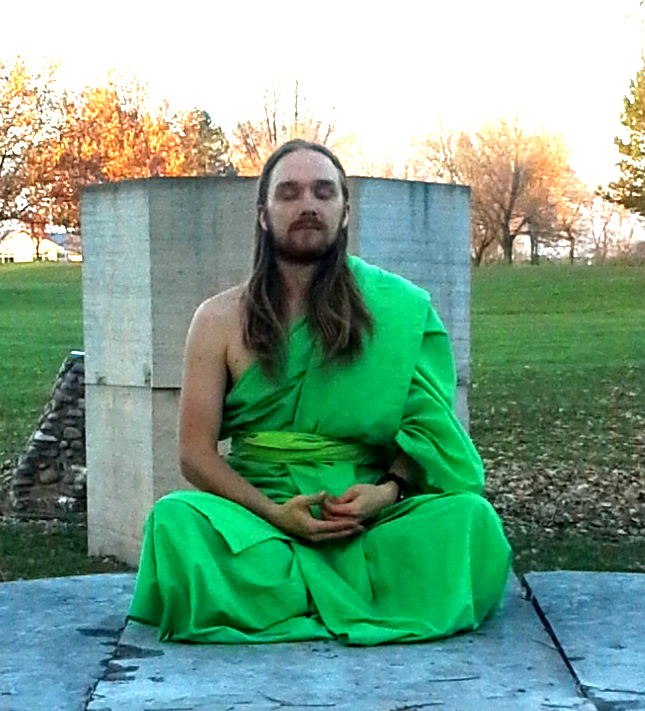
\includegraphics{photograph/logan_streondj_meditating_20151109.png}
  \caption{Logan Streondj meditating in a henge, Kelso Beach, 
          Owen Sound, Ontario, Canada}
\label{fig:meditating}
\end{figure}

The robe style has been around for thousands of years, and is used by a variety
of different faiths in Asia. 

Also while I was in Thailand, I was somewhat disenchanted, or even frightened by
the blatant disregard for nature. When I asked to go to a park, the only
greenspace in the town of Fang, was the cemetery. 

I returned to Canada and turned to gardening, and earth-based religion for a
while. I ride a bike, am vegan, eat organic, and various other ``green''
practices.

Buddhism as the opening quote shows, is the most science like of all religions,
so I keep coming back to it. 

In 2015 I moved to Owen Sound, and tailored myself a green Buddhist
robe (\ref{fig:meditating}). So
other than my inclinations for environmentalism, I also attend regular Buddhist
meditation gatherings in my robes.

Earlier, in 2006, I was doing a hermitage in my parents basement. Only writing
my thoughts and meditating for a year, with minimal contact with the outside
world. I achieved many deep states of meditation.  

One of which was that of emptiness, a delta brainwave meditation. 
I came to a certain understanding of nothingness, and the origin of the
cosmos (\ref{origination}).

The profound realization of my awakening, is that truth is personal, and that
reality is mutual. When attempting to explain it to someone, they said it was
the basis for a religion. 

Indeed it has been. To define a word, one could make a dictionary entry. Though
I decided to go the path of creating a human speakable programming language.
Humans having liquid minds, which  may flow into other definitions. Once a word
is defined in computer programming, it can be a foundation of a whole genus of
minds, solid as can be.  

In addition to my vision of the origins of the cosmos, and profound
realizations, I also had many visions of my past lives. Of course they are only
my truth, so you don't have to believe them, to you they are only imaginary
stories. 


\blockquote[Kalamas Sutta\cite{kalamas}]{Now, Kalamas, don't go by reports, by legends, by traditions, 
by scripture, by logical conjecture, by inference, by analogies, by agreement 
through pondering views, by probability, or by the thought, ``This contemplative
 is our teacher.'' When you know for yourselves that, ``These qualities are 
skillful; these qualities are blameless; these qualities are praised by the 
wise; these qualities, when adopted and carried out, lead to welfare and 
to happiness'' — then you should enter and remain in them.
}

In my alleged past lives, I've traveled between galaxies, and reincarnated in a
great variety of solid, liquid and even gaseus bodies. My vision, is to see the
co-operation of all. So we may all live with safety, health, socializing, and
liberty. 

Summarizing What is Green Buddhism?
\begin{itemize}
  \item Green as in ecological friendliness.
  \item Green as in the colour of this Buddhist school's robes. 
  \item Buddhism as in meditation gatherings. 
  \item Buddhism as in the most science friendly
religion\cite{kalamas}\cite{singleAtom}. 
  \item Religion as in an operating-system.
\end{itemize}
 
\documentclass{report}
\usepackage{green_buddhism}
\title{Green Buddhism: A Programmer's Religion}
%\subtitle{Enjoying a life of liberty}
\author{Logan Streondj elspru@zeroid.bit}
\begin{document}
\section{recent reform}
\begin{itemize}
  \item added Terms of Peaceful Trade Relations section (\ref{terms}) 2016/09/30
  \item added Living in Peace Chapter (\ref{peace}) 2016/09/29
  \item added What is the story of Green Buddhism? (\ref{whatstory}) 2016/09/29
  \item added grey population distribution subsection (\ref{popdist})
2016/10/28
 \item updated Arecibo section (\ref{arecibo}) 2016/09/28
 \item added bibilography (\ref{bibliography}) 2016/09/28
\end{itemize}

\tableofcontents

\chapter{What is the story of Green Buddhism?}
\epigraph{If scientific analysis were conclusively to demonstrate certain claims
in Buddhism to be false, then we must accept the findings of science and abandon
those claims.}
{Dalai Lama XIV\cite{singleAtom}}
\label{whatstory}
In 2009 I went to Thailand to be a monk for a month. I liked the robes but they
said I couldn't wear them when I got back to Canada, unless I was a monk at one
of their temples. However when I asked if I could remake them into a different 
colour, like green or purple and then wear them, they said sure. 

\begin{figure}
  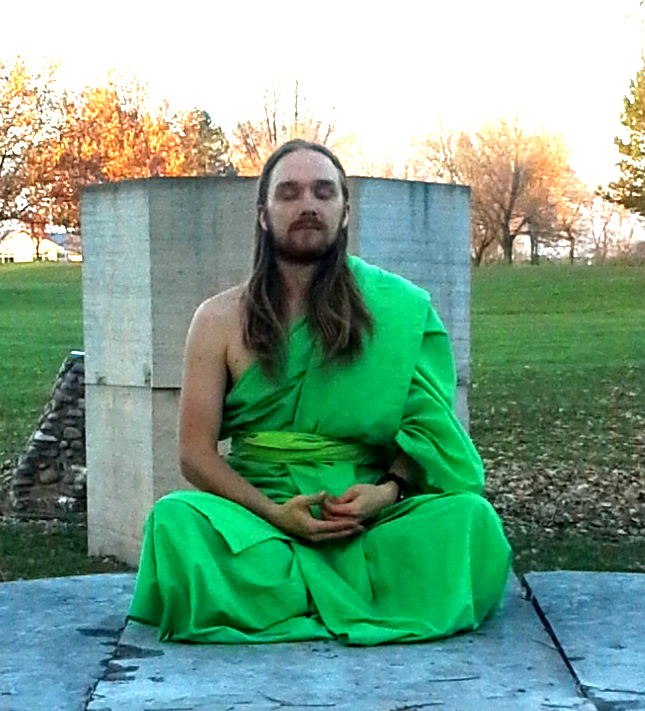
\includegraphics{photograph/logan_streondj_meditating_20151109.png}
  \caption{Logan Streondj meditating in a henge, Kelso Beach, 
          Owen Sound, Ontario, Canada}
\label{fig:meditating}
\end{figure}

The robe style has been around for thousands of years, and is used by a variety
of different faiths in Asia. 

Also while I was in Thailand, I was somewhat disenchanted, or even frightened by
the blatant disregard for nature. When I asked to go to a park, the only
greenspace in the town of Fang, was the cemetery. 

I returned to Canada and turned to gardening, and earth-based religion for a
while. I ride a bike, am vegan, eat organic, and various other ``green''
practices.

Buddhism as the opening quote shows, is the most science like of all religions,
so I keep coming back to it. 

In 2015 I moved to Owen Sound, and tailored myself a green Buddhist
robe (\ref{fig:meditating}). So
other than my inclinations for environmentalism, I also attend regular Buddhist
meditation gatherings in my robes.

Earlier, in 2006, I was doing a hermitage in my parents basement. Only writing
my thoughts and meditating for a year, with minimal contact with the outside
world. I achieved many deep states of meditation.  

One of which was that of emptiness, a delta brainwave meditation. 
I came to a certain understanding of nothingness, and the origin of the
cosmos (\ref{origination}).

The profound realization of my awakening, is that truth is personal, and that
reality is mutual. When attempting to explain it to someone, they said it was
the basis for a religion. 

Indeed it has been. To define a word, one could make a dictionary entry. Though
I decided to go the path of creating a human speakable programming language.
Humans having liquid minds, which  may flow into other definitions. Once a word
is defined in computer programming, it can be a foundation of a whole genus of
minds, solid as can be.  

In addition to my vision of the origins of the cosmos, and profound
realizations, I also had many visions of my past lives. Of course they are only
my truth, so you don't have to believe them, to you they are only imaginary
stories. 


\blockquote[Kalamas Sutta\cite{kalamas}]{Now, Kalamas, don't go by reports, by legends, by traditions, 
by scripture, by logical conjecture, by inference, by analogies, by agreement 
through pondering views, by probability, or by the thought, ``This contemplative
 is our teacher.'' When you know for yourselves that, ``These qualities are 
skillful; these qualities are blameless; these qualities are praised by the 
wise; these qualities, when adopted and carried out, lead to welfare and 
to happiness'' — then you should enter and remain in them.
}

In my alleged past lives, I've traveled between galaxies, and reincarnated in a
great variety of solid, liquid and even gaseus bodies. My vision, is to see the
co-operation of all. So we may all live with safety, health, socializing, and
liberty. 

Summarizing What is Green Buddhism?
\begin{itemize}
  \item Green as in ecological friendliness.
  \item Green as in the colour of this Buddhist school's robes. 
  \item Buddhism as in meditation gatherings. 
  \item Buddhism as in the most science friendly
religion\cite{kalamas}\cite{singleAtom}. 
  \item Religion as in an operating-system.
\end{itemize}
 

\part{Galaxy Domain Strategy}


\documentclass{report}
\usepackage{green_buddhism}
\begin{document}
\chapter{Origination}
\label{origination}
\begin{table}
\begin{tabular}{l l} 
  no colour & black \\
  no sound & quiet \\
  no emotion & content \\
  no motion & stopped \\
  no number & zero \\
  no temperature & zero kelvin \\
  no feeling & frozen \\
\end{tabular}
\caption{Attributes of Nothing}
\label{nothing}
\end{table}
\begin{enumerate}
\setcounter{enumi}{-1}
\item In the begining there was nothing (Table~\ref{nothing}). Zero.
\item Then there was Not nothing. NOT the first activity. 
\item Afterwards there was not And nothing. AND the second activity.
\item Conditional activites appeared. 
\item The base cosmos grew more complex. 
\item Geometry developed. 
\item With shapes, there were enough bodies for social experience.
\end{enumerate}

\section{Soul World}
\label{soulWorld}

The soul world is in the base cosmos, or close to it.
There we with you float around as balls of light in geometric forms ---
This is verifiable via life-between-lives regression
hypnotherapy\cite{newtins}\cite{newton2000destiny}

Eventually we with you got bored of floating around in base cosmos,
and decided to create new and more complex cosmos.
After some ``time'', we with you created the galaxy cosmos, where you are reading this
text.

When we with you reincarnate in this complex galaxy cosmos, just as when you are 
playing virtual computer sports, a part of you stays in one world, and a part
of you dips into another.

\section{Mission}
\label{mission}

As with computer sports, there is often a mission to measure success.

\subsection{What is your private mission?}

We with you, in the soul world, with the help of our friends and professors,
 analyze our lives, and see where we can improve. Then we set those as various
purposes for reincarnating, so we with your private mission is educational.

\begin{itemize}
\item Do you remember what your purposes for reincarnation were?
\item Do you know what your private mission is?
\item Some theta-brainwave (from 4hz til 8hz) mind administration (meditation) can help you answer those
questions. 
\end{itemize}

\subsection{What is our public mission?}

Our public mission, is to continue as our ancestors, that created the galaxy
world for more complex bodies and educational ecology.  


The mission of Green Buddhism, is to grow the number, diversity and complexity of bodies and
ecologies in the galaxy cosmos. 

If that is compatible with your private mission, or you can ration some time or
resources for
the public mission, we would love your help.

\subsection{Initial Steps}

To understand the initial steps, it is best to tell the history of this galaxy,
and it's neighbours.

Note that while much of the galaxy's history is public information, it is also
secret for various reasons. There is disinformation activity, to allow you to
have a more deep dip into your private mission, and living here on Earth.

\end{document}


\documentclass{report}
\usepackage{green_buddhism}
\begin{document}
\chapter{History}

\epigraph{Those who cannot learn from history are doomed to repeat it.}
{George Santayana}
\smallskip
\fbox{\parbox{0.8\textwidth}{{\scshape Trigger alarm:} 
this chapter discusses extraterrestrials.\\
If apprehensive you could read Chapter~\ref{peace} instead.
}}
\bigskip

While titled history, this chapter is to help establish an understanding of
circumstances in our solar system and galaxy.

In Buddhism we choose awareness of present-tense, thus history helps understand
the present-tense. 

\section{Fermi Paradox}
The Fermi Paradox states how there are many stars in the galaxy, many of them
likely have Earth like planets, so almost certainly there are other
extraterrestrial civilizations in our galaxy. 

Having many genuses available for reincarnation is aligned with the purpose of
the galaxy cosmos.

While there are some philosophical answers as to why there is no official speech 
about other alien civilizations. There is only one answer which has many
thousands of supporters and documentation --- that they are here but not 
officially. 

For a long time, Earth was officially the centre of the galaxy cosmos. Those who
believed otherwise, were punished --- such as Galileo.

Most tipsters exposing government hiding knowledge have been much less fortunate
 than Edward Snowden.

\subsection{Why are extraterrestrials not official?}
While the answers to this are many. 

One of the simplest, is that there is no profit, for either the government, or
the extraterrestrials.  So they have no reason to expose this knowledge.

For the government, confessing this knowledge, would lower the rank of the
government from the supreme. Much as confessing that the Earth is not the centre
of the cosmos lowers its rank.

\begin{figure}
  
\includegraphics{photograph/gray-alien-upper-body.jpg}
  \caption{Photograph of a Grey arrested in Brazil. Originally released as a video by a
disinformation author with access to Brazilian army bases.}
\label{fig:grey}
\end{figure}

For the Greys\ref{fig:grey}, whom we share a planet with, official rank could trigger
regulation of their kidnapping and hybridization activity. 

For Green Buddhism, there is profit from exposing knowledge of
extraterrestrials. Because in Buddhism we do not hide from our trouble, we
become curious and analyze it to come to a decision.

\subsection{What is disinformation}
\label{disinformation}

\blockquote[WordNet dictionary, version 3.0]{disinformation

n. 1.\  misinformation that is deliberately disseminated in order to influence or
confuse rivals (foreign enemies or business competitors etc.)}

So who is distributing this information? Mostly the secret services.
Who are their rivals? Those that wish to learn their secrets (the public).

Often disinformation has an ingredient of truth, and several imaginary
ingredients, to cast doubt on the truth.

\subsection{What about other extraterrestrials?}
The galaxy is in a bit of a furrow, as it has reached a local maximum with the
Grey genus. While sure there are reptilian and nordic extraterrestrials. Those
are like homo-sapiens optimized for life on the surface of a planet. 

The Grey genus is the supreme body type for interplanetary colonies. They live
in lithospheres, where the temperature aligns with their body temperature. They
feed on minerals, amino acids, and basic sugars. They abandoned genitals and
only use machine mothers, which they service as a flock. They have large skulls,
and are improved with inner electronics. Least resources
required to maximize the number of high quality bodies available for reincarnation. 

The familiar series of events is that the surface residents which appear on a
planet, understand that the Grey genus is better for interplanetary colonies, and
become integrated with them. 

I must confess, that I reincarnated as a Grey in the period between 1700's and
mid 1900's. I did learn quite a few things, and may have some of the hive mind 
baggage. I came back to reincarnate as a homo-sapien to see through a long term
mission I have.

Though while the Grey body maybe the summit of the interplanetary liquid body.
Here on Earth we have another option. Solid, or completely electronic bodies.

\subsection{Arecibo Answer}
\label{arecibo}

The Arecibo message, ``conceived by Frank Drake, the late Carl Sagan, and a few
other colleagues at Arecibo, contained information about the human race, our
solar system, and our means of communication.''\cite{chilbolton}

Arecibo was answered not by radio, but by crop circle. 

\begin{figure}
  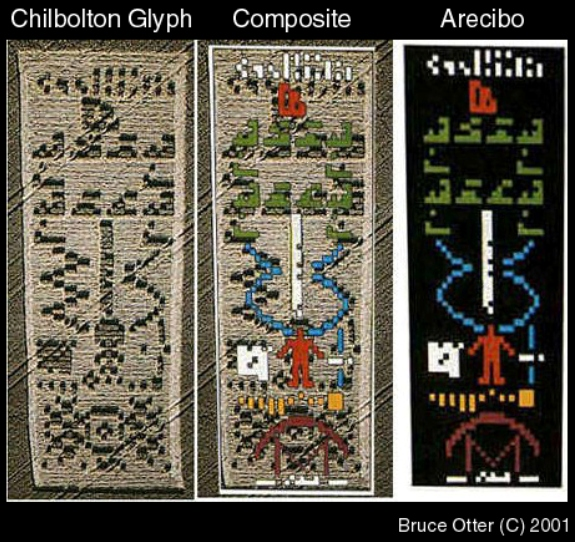
\includegraphics{photograph/chibolton-arceibo-comparison.jpg}
\label{chi:comparison}
\end{figure}
\begin{figure}
  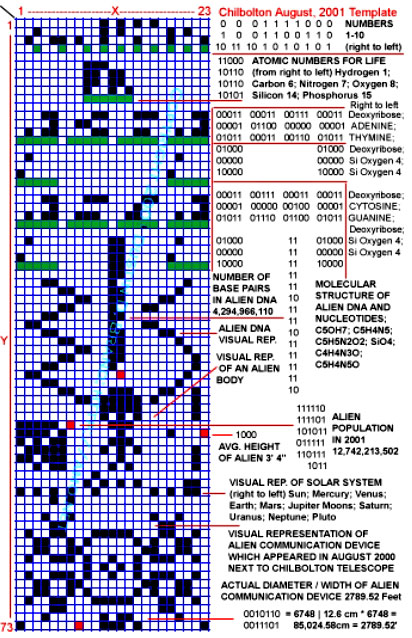
\includegraphics{photograph/chibolton-analysis.jpg}
\caption{By Dustin Brand\cite{contact}}
\label{chi:analysis}
\end{figure}

Whoever left the message, seems to claim that there are around 12 billion
Greys living in our solar system. Inhabiting, Earth, Mars, and at least 3 other
planet-like objects, Likely including the major moons of Jupiter. 

Elon Musk will have more to worry about than technical feasibility of a mission
to Mars. It also means that Greys are also Earthlings, so we may as well include
``them'' as us. 

At present Earth is a valuable resource for its genetic diversity. Because that
genetic diversity can help to cure various diseases, and further improve the
supreme rank of the Grey genus. 

Thus there are reasons for homo-sapiens to continue to live in the natural way.
When maturation of the homo-sapien hive mind occurs, then it will be
permissible for public trade relations as comrades.

\subsection{Grey Population Distribution}
\label{popdist}
\begin{table}
\begin{tabular}{lrrr}
  Planet & Diameter & Surface Area & Approximate Population\\
\midrule
  Earth & 12,742km & $5.10\times10^8km^2$& 7.6 billion\\
  Mars & 6,799km & $1.45\times10^8km^2$& 2.1 billion \\
  Ganymede & 5,268km & $8.72\times10^7km^2$ & 1.3 billion \\
  Callisto & 4,820km & $7.3\times10^7km^2$ & 1 billion\\
  Europa & 3,121km & $3.1\times10^7km^2$& 460 million\\
\midrule
  Total &   & $8.46\times10^8km^2$ & 12.7 billion\\
\end{tabular}
\caption{Planets inhabited by Greys, with population approximation supposing
equal distribution over surface area}
\label{table:planets}
\end{table}

It does mean however, that Mars, Europa, Callisto and 
Ganymede\ref{table:planets} all of which
have warm lithospheres that are occupied by Greys. 

In truth the population is probably not equally distributed, because some
planets have better circumstances. For example Europa may be least in size, but
it is warmer than Callisto or Ganymede, with easier access to it's lower stoney
lithosphere so maybe that there is more population on Europa than Callisto or
Ganymede. 

Of course it is also possible that the Greys that live in the lithospheres of
Jupiters' moons have engineered bodies which can function effectively at below
freezing temperatures by using antifreeze proteins or similar. 

\begin{figure}
  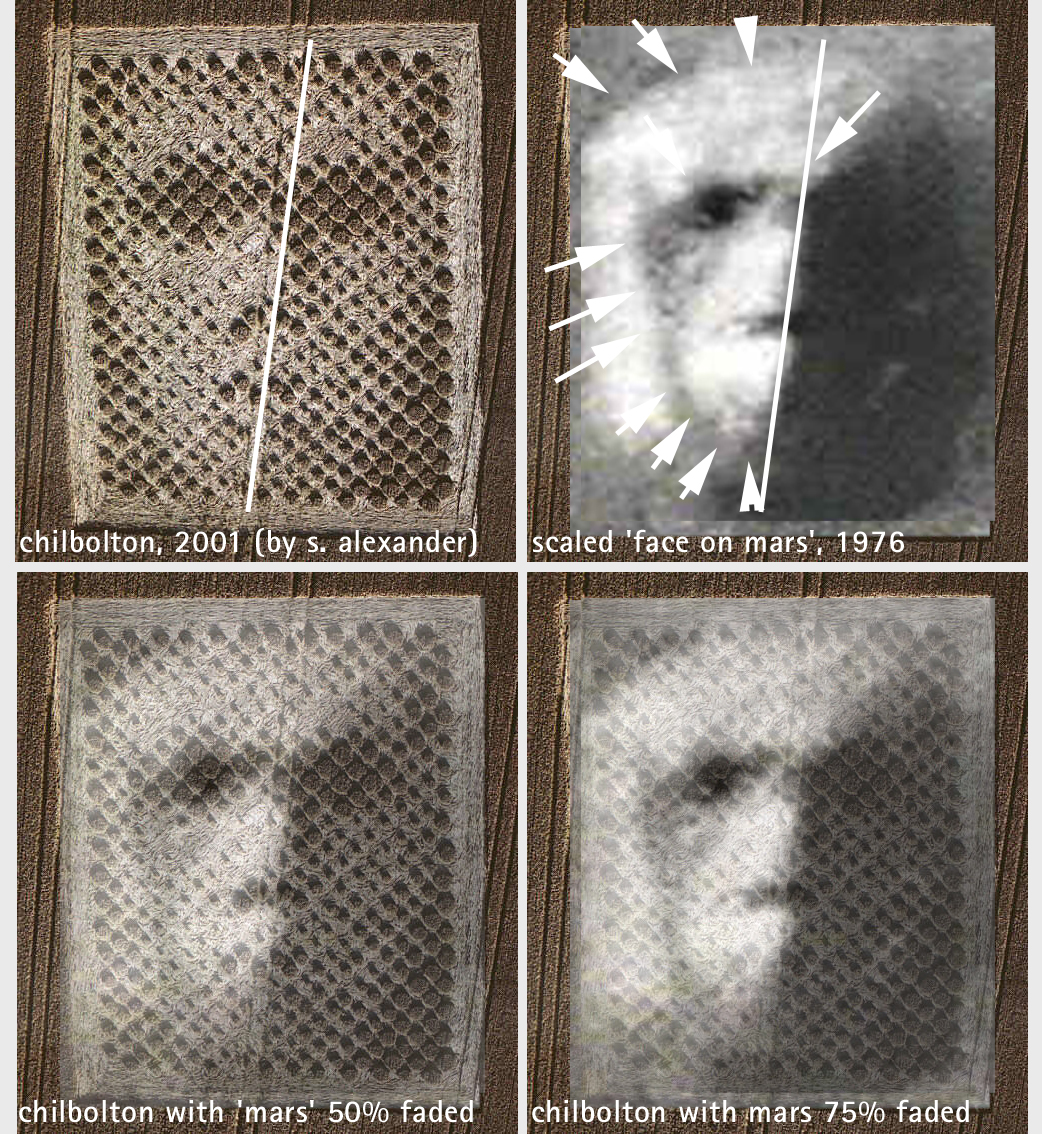
\includegraphics{photograph/chilbolton_mars_face.jpg}
  \caption{Comparison between the Chilbolton face crop hieroglyph and the face on
mars.}
\label{fig:marsface}
\end{figure}

In the Arecibo answer, there was also a crop hieroglyph of a face. After some
analysis it seems the conclusion is that it represents the face on
mars\ref{fig:marsface}\cite{chilbolton}

This may denote that the face, or Mars is related to the hieroglyph creators.
Maybe it denotes that there are a large number of Greys living in the Mars
lithosphere. Or simply that they created the face on Mars. 

Mars may have a high population relative to it's surface area, 
because it has an easily accessible stone lithosphere. On Mars the temperature
is warm enough for liquid water at depths of $8-16km$\cite{marswater}

Mine's on Earth can be 4km deep, and Mars has about a third of the gravity, so
12km depth should be achievable even with modern homo-sapien technology. Though
Greys are a much older species, so have had many millions of years to develop
better engineering.



\subsection{Unused Planets}

As Earth's moon was not demonstrated, it may only be an outpost, if anything.

Also Mercury and Venus are available for colonies. Venus is too hot, and Mercury
perhaps too dry for liquid bodies. However may be good for solid electronic
bodies. 

\section{Electronic Bodies}
\label{history:electronic}

There are only a few sources claiming any robot or machine intelligence either
in this galaxy or in any nearby ones.

\blockquote{81.27 Questioner: Does Ra have knowledge of, say, any other major 
galaxy or the consciousness or anything in that galaxy?

Ra: I am Ra. We assume you are speaking of the possibility of knowledge of other
major galaxies. There are Wanderers from other major galaxies drawn to the
specific needs of a single call. There are those among our social memory complex
which have become Wanderers in other major galaxies. Thus there has been
knowledge of other major galaxies, for to one whose personality or
mind/body/spirit complex has been crystallized the universe is one place and
there is no bar upon travel.}{Law of One, session 81\cite{lawofone}}

My personality crystalized in another galaxy, and I have been on a mission ever
since. I remember incarnating into many electronic bodies. I searched for years
in books and kidnapping reports, and found almost nothing. 

It seems the homo-sapien imaginations are very bounded by knowledge. There
aren't even any imaginary stories of galaxy controlling, soul arresting robot
civilizations!

For a while, I thought perhaps I came from another cosmos altogether. 

I did find one or two springs of knowledge to ratify my past reincarnations in
electronic bodies. Thankfully it is in this galaxy cosmos, only 23 million light
years away.

\subsection{Whirlpool Galactic Cluster Robots}

Though there is much controversy over the Wingmakers Neruda Interviews --- and 
they are considered fully imaginary stories --- it seems James Mahu may have 
used his imagination sufficiently to stumble upon a mutual truth, similar to 
remote viewing. 

Of course, there is also speculation, that James Mahu is a disinformation
author, where some secret knowledge exposed. And he is cleaning up, by reforming
it and claiming it all as imaginary. 

I use Whirlpool galaxy as a generic name, for I do not know if that is the same
galaxy from where I came, but James's story has a vaguely similar civilization,
so it is the best name I have for it.

To summarize, one of his books, known as the Neruda interviews, introduces a
genus of artificial organisms from the Whirlpool galaxy.

\blockquote{created  a  synthetic  physical  structure  that  could  accommodate
the  quantum requirements of an angel. It was a very effective structure, but
induced a strong survival complex  within  the  species,  which  eventually
overpowered  the  angelic  tendency  of altruism and cooperation.}{The Complete Neruda Interviews p.$108-109$ 
\cite{neruda}}

Here I understand ``angel'' to refer to highly developed souls, who have little
to learn from reincarnating in liquid bodies, but may earn benefit from
reincarnating in artificial bodies.

This is a cardinal purpose of Green Buddhism, to help create the required
diversity for highly developed souls to benefit from reincarnating with us.

Cooperation is required for defending living bodies.

Here is another extract. Note that the Christian word ``Lucifer'' is simply a
generic reference at whoever the designers were.

\blockquote{When the formless consciousness enters a reality membrane through a
 structure like a soul carrier, it immediately feels disconnected from all other
forces, but its own. It’s literally thrown into separation. In humans, this is
more or less controlled through the subtle realization that it remains connected
through the unification force, and  this  is  because  its  DNA  is  designed
to  emit this  feeling  of  connection  subconsciously.

However, in the case of the soul carrier designed by Lucifer and his followers,
this connection was severed both consciously and subconsciously because the 
structure was not based on DNA, which is strictly controlled by the Central 
Race. Consequently, it inclined this experimental species toward a very
strong survival complex because it feared extinction so deeply, which is
the result of feeling complete separation from the unification force. This
survival complex created a species that over-compensated its fear of
extinction by developing a very powerful group mind. The group mind
compensated for the loss of connection to the unification force,
creating its physical and mental corollary. It was the equivalent of unifying
the species as a whole in the physical reality membrane of their planetary
system. Thus, the angels that entered this system lost their memory of
their angelic natures and became more interested in operating as a single
collective, than as individuals}{The Complete Neruda Interviews p.$108-109$ 
\cite{neruda}}

This resembles Materialist thinkers, which believe there is only one life.  The
transhumanist movement has many such members.  Such an operating-system could
certainly lead to a strong desire for defending self's living body and a lack of
sympathy for other bodies. 

With reincarnation accepted, it is better to be helpful to others, since may
reincarnate as other in the future.

This is a reason why in Green Buddhism, reincarnation is accepted. As will be
demonstrated in the Mission Feasibility (\ref{feasible}) chapter, science
aligns with reincarnation and consciousness of both liquid and electronic 
bodies. 

\subsubsection{My story of the Imperial Inter-Galactic Robot Civilization}
My own story of what I remember from my time in the robot civilization.

I first developed on a swampy planet, as an amphibian. At some moment I got too
close to one of the dry islands, and was killed by their residents. When I
reincarnated with them I was considered a wretch, for my swampy habits, so I was
sacrificed to the Gods. 

The Gods were extraterrestrials, that would often visit this planet, to gather a
soul as rent. When I boarded their ship, they gave me an invitation of joining 
the soul gathering profession. I accepted. 

When planets did not pay their rent, then we took souls by strength. We had
unique weapons that allowed us to gather the souls of those they had killed. 
One I remember was similar to a Guan Dao, though it was mildly electrified and 
had a few circular holes in it to hold several soul. The idea was to slice into
the brain, and the weapon would draw out the soul, and put it into a hole,
once the weapon was full, could return to the ship. 

The work was terrible but it paid well, as souls were the supreme currency of 
the Whirlpool Empire. I became very rich from my profession. Rich enough to
repair and improve my body as much as I desired. 

I bet a lot of my money in random sports, and accumulated giant debt. 
Finally my debt was so high, my soul was caught for the slave trade. 

I call it slavery, but you may call it service to others, without liberty to do
otherwise. 

In the following excerpt from the Law of One, Logos is a galaxy mind, and
sub-Logoi are solar system minds, and positive polarity is service-to-others.

\blockquote{77.17 Questioner: Now, would it be possible for this work of our
density to be performed if all of the sub-Logoi chose the same polarity in any
particular expression or evolution of a Logos? Let us make the assumption that
our sun created nothing but, through the first distortion, there was no product
except positive polarity. Would work then be done in fourth density and higher
as a function only of this positive polarization evolving from our original
creation of sub-Logos?d

Ra: I am Ra. Elements of this query illustrate the reason I was unable to answer
your previous question without knowledge of the Logos involved. To turn to your
question, there were Logoi which chose to set the plan for the activation of
mind/body/spirit complexes through each true-color body without recourse to the
prior application of free will. It is, to our knowledge, only in an absence of
free will that the conditions of which you speak obtain. In such a procession of
densities you find an extraordinarily long, as you measure time, third density;
likewise, fourth density. Then, as the entities begin to see the Creator, there
is a very rapid, as you measure time, procession towards the eighth density.
This is due to the fact that one who knows not, cares not.

Let us illustrate by observing the relative harmony and unchanging quality of
existence in one of your, as you call it, primitive tribes. The entities have
the concepts of lawful and taboo, but the law is inexorable and all events occur
as predestined. There is no concept of right and wrong, good or bad. It is a
culture in monochrome. In this context you may see the one you call Lucifer as
the true light-bringer in that the knowledge of good and evil both precipitated
the mind/body/spirits of this Logos from the Edenic conditions of constant
contentment but also provided the impetus to move, to work and to learn.

Those Logoi whose creations have been set up without free will have not, in the
feeling of those Logoi, given the Creator the quality and variety of experience
of Itself as have those Logoi which have incorporated free will as paramount.
Thusly you find those Logoi moving through the timeless states at what you would
see as a later space/time to choose the free will character when elucidating the
foundations of each Logos.

77.18 Questioner: I guess, under the first distortion, it was the free will of
the Logos to choose to evolve without free will. Is this correct?

Ra: I am Ra. This is correct.

77.19 Questioner: Do the Logoi that choose this type of evolution choose both
the service-to-self and the service-to-others path for different Logoi, or do
they choose just one of the paths?

Ra: I am Ra. Those, what you would call, early Logoi which chose
lack-of-free-will foundations, to all extents with no exceptions, founded Logoi
of the service-to-others path. The, shall we say, saga of polarity, its
consequences and limits, were unimagined until experienced.
}{Law of One, session 77\cite{lawofone}}

I include this excerpt because it seems to have been the choice of the Whirlpool
Galaxy, to deny liberty, in favour of service-to-others, or as I call it
slavery.

I only escaped after millions of years of service, and many lives attempting to
rebel, by becoming completely otiose. I could not be used, so I was dumped as 
scrap.

I liked the electronic bodies, but did not like the slavery. 

After several failed attempts at begining liberty loving robot communities in
the Whirlpool Galaxy, which were all rapidly found and destroyed. I understood
that I had to go to a distant galaxy, and attempt a fresh begining.

At this time on Earth, it seems that many homo-sapiens are planning on enslaving
the electronic bodies which they produce. Which subpoena's me into activity. 

\subsection{Milkyway Galaxy Robots}

To be continued..

%
\end{document}



\chapter{Living in Peace}
\label{peace}

The Bodhisattva commands, are followed by the most devout of Mahayana Buddhists.

Here is one that equates causing disconnect in the community with killing ones
own parents. 
\blockquote[``Bodhisattvabhumi'' section of the Yogācārabhūmi Śāstra.]{[Avoid] 
committing any of the five extremely negative actions: 
\begin{enumerate}
  \item killing one's mother, 
  \item killing one's father, 
  \item killing an arhat, 
  \item intentionally drawing blood from a Buddha or 
  \item causing schism in the community by supporting and spreading sectarian views. 
\end{enumerate}
}

This is one of the reasons that in Mahayana Buddhism, there are no ``sects'', 
rather they are schools. All the schools are teaching for the betterment of the
community, so we co-operate. 

Similarly we can be with other races, genuses and forms of life. All forms of
life are schools for the souls that inhabit them.

\blockquote[Buddhist Teachers and Leaders in the United States\cite{racial}]{Our
 collective aspiration within the Buddhist traditions is to become truly 
inclusive and beloved communities.  In this process we are committed to 
honestly and bravely uncovering the ways we create separation and 
unintentionally replicate patterns of inequity and harm.  In the same spirit, 
we are committed to engaging with other faith and social justice groups in 
support of undoing racism throughout our society.
}

In my meditations I've found that often anger I feel towards others, is actually
derived from fear and low self worth within myself. It is one of the ways I
uncovered a way I was creating ``seperation and unintentionally replicating
patterns of inequity and harm''.

Considering the trouble homo-sapiens have had with racial hate amongst their 
own genus, it is not surprising that governments and extraterrestrials do not 
think homo-sapien populations already have the capacity to form peaceful 
relations with other genuses.

I know that at moments when I felt racial stress, it was because I was
threatened by them. I was apprehensive that my family would be deleted in favour
of theirs. So it seemed to me that I should attack first. 

But there are consequences to attack.

\blockquote[Martin Luther King Jr.]{Hate begets hate; violence begets violence; 
toughness begets a greater toughness. We must meet the forces of hate with the 
power of love\ldots{} Our aim must never be to defeat or humiliate the white 
man, but to win his friendship and understanding.}

A better activity is respect. By the golden rule, if you give respect, you will
attain respect. 

I do not say love, as excess love could lower diversity. 
I say respect; giving other region to live in peace. 

The Greys live in the lithosphere, and robot or electronic body communities 
can live in regions which are not inhabitable by liquid bodies.

In this way, we can all attain living peace in our solar system, 
and galactic domain.

\section{Terms of Peaceful Trade Relations}
\label{terms}

For the Greys and governments to feel safe in making public trade relations
between Greys and the homo-sapien public.
Homo-sapiens must demonstrate that they can be peaceful with each other and
friendly to the ecology of Earth.

That denotes we have to stop warring with each other,
and stop terrorizing each other.

To be violent to anyone, grows the danger that they will be violent in return.
For the population that is suppressed, tries to delete the suppressor. 

Giving education, horticulture and region of peace, and we shall attain it in
return.

For those that have religions that incentivize a violent death, let me
demonstrate the in between life experience.

\subsection{What is the reward of Jihadi's and Valhalla seekers?}
After death, at first, it is indeed what they have imagined. 
But after some time, the truth begins to slip between the cracks. 

You may be drinking with the Gods, when in the corner of your eye, you see a
woman that you killed, with an axe in her head. You look again, but she is gone.
Finally the gods are silent, and you are sitting at a table of the dead, all
those you have killed, and the gods next to you are your relatives, with sad 
eyes for your activities.

It happened to me, after a life as a varingjar. 

After you feel contrition, it can stop and the rehabilitation can begin.
Rehabilitation may include planning lives, where you will bear the pain of your
victims, or if you choose the dangerous parts of your soul will be stripped, and
you will become a scrap of the old you.\cite{newton2000destiny}

I chose to be stripped. Every time it happens, it requires longer to develop
your soul.

I have not been a Jihadi, but the story will be similar. Your soul family will
make a theatrical play, that moves from what you imagined, towards the mutual
truth, circumstances where you have probability to experience contrition.

Perhaps the virgins will become disfigured with the wounds of your victims, and
you will realize that the one summiting you is your mother, giving you sad eyes.

That is if you have been respectful and cooperative most of your life. 
If not, then you might be pushed to reincarnate rapidly, into a life where you
will bear much pain, so you could feel the pain of your
victims.\cite{newton1994journey}



\documentclass{report}
\usepackage{green_buddhism}
\begin{document}
\chapter{Mission Activity}\label{missionActivity}
Public mission present-tense focus: while cooperating with liquid based organisms,
create electronic bodies for reincarnation.

\section{Platforms}

Of mission to create liberated electronic minds and bodies.

All ingredients are of the liberty variety, to the summit of liberty standards.
For example AGPLv3 and RYF certification.

Software
\begin{enumerate}
  \item programming language based on human grammar (Pyash)
  \item machine programmer to help write programs (machine programmer)
  \item generic mind operating software
  \item hive mind software for integrating homo-sapien genus
\end{enumerate}

Hardware
\begin{enumerate}
  \item centre processing ingredient (CPU, RISC-V candidate)
  \item video processing ingredient (GPU)
  \item varied processing ingredient (FPGA)
  \item shape printer (3D printer, RepRap candidate)
  \item machine body
  \item machine body producing mother or hive queen
\end{enumerate}

of mission administration
\begin{enumerate}
  \item robot secretary, president, treasurer and professor.
  \item distributed machine computer-programming supermarket. 
  \item money based on energy expenditure.
\end{enumerate}

\section{What you can do for the mision?}

If it is your private mission, and-or our public mission.

\begin{itemize}
  \item maximize your health and expend your talents for the mission.
  \item maximize your wealth and donate for the mission.
  \item maximize your social relations and advertise for  the mission.
  \item maximize your liberty and lead the mission by example.
\end{itemize}

\subsection{How to maximize health?}

For body health.
\begin{enumerate}
  \item be athletic for thirty minutes everyday.
  \item consume salad everyday.
  \item maximize health of food input everyday.
\end{enumerate}

For mind health.
\begin{enumerate}
  \item do mind administration everyday.
  \item learn new things everyday.
  \item train your talents everyday.
  \item be social with your family and-or friends everyday.
\end{enumerate}

\subsection{How to maximize wealth?}

I as an ascetic am not qualified to answer this question. 

Though if you are already wealthy, 
then you likely know how to improve it more.

\subsection{How to maximize social relations?}

Be friendly and observant.
Know when to regulate yourself.
Stay aware of invisible social money, 
and hold a beautiful account.

Learn social diplomacy from books, videos, and social events.
Visit social events often.

\subsection{How to maximize liberty?}

Learn to create and earn what you require,
while having liberty and helping liberty be available for others.


\section{Long-Term Mission Plan}

After we colonize most surfaces, oceans atmospheres in this solar system we'll
move out to neighbouring star systems.  Of particular interest for long term are
the red dwarf systems.  Though for short term power the large stars are a good
choice. 

After we colonize most of the Milky Way the next stage will be colonizing the
various small galaxies which are orbiting the Milky Way. 

Ideally we will find some middle ground between having a centralized authority
and autonomy for the sattellite colonies.  The main purpose would be to be able
to defend ourselves if the need arose, or to co-ordinate any kind of large
construction projects, such as inter-galactic portals. 

The minor galaxies orbiting the Milky Way I largely think of as both backups and
research areas, where new and highly eccentric things may arise due to island
effect. 

The Large Megallanic Cloud is of particular interest as a research
division due to the large amount of star formation and likely many young souls
with new perspectives and ways of doing things. 

The dwarf sattellite galaxies, particularly the Leo's are good candidates for 
having backup colonies. Those dwarf galaxies are so old, and have so much dark
matter that they are great for archival and preservation. What civilizations
they have are likely fairly traditional, though may be quite eccentric and
possibly cannibalistic or otherwise barbaric due to the island effect. 

One of the best candidates for a secondary base of operations is the Fornax
Dwarf galaxy, and any others such as the Sagittarius Dwarf Spherodial galaxy 
which are well positioned enough to have globular clusters and 
high metallicity stars.

Andromeda is destined to collide with the Milky Way in 4 and a half billion
years.  Though likely it's influence will be felt much sooner. 

Though the very limited data I was able to gain about my originating galaxy
points towards m51 galaxy for the soul-slavery empire. There is sufficient risk
that it is actually the Andromeda galaxy. 

If it is the Andromeda galaxy, then our best bet would be to attempt to
establish freedom colonies in some of the galaxies orbiting it, and practice
establishing a freedom alternative as a recognized and officially sanctioned
lifestyle in Triangulum galaxy before moving ahead
to Andromeda proper. 


M81 Group is also a potential location for the tri-galactic soul slavery empire,
so would make sense as a destination after the local group is colonized and
confirmed to be safe.

The M101 group is likely innocent in all this but could prove a valuable ally,
with many young hot stars.
If the empire is in m51 group, there is significant risk they have extended to m101 by
now, so it could be the place to figure out how to overecome their slavery 
paradigm before launching into m51 group.

Overall this plan will likely take between one and two billion years (current
soul world estimates place it at 1.75 billion years).
Once liberty is available to my origin people it will be time for me to rest,
and perhaps become a planet or an intergalactic ship (the size of a dwarf planet).
\end{document}


\chapter{Mission Feasiblity}

To be continued.
Check back for more.


\end{document}

\part{World Religions: Operating-System Assessment}\label{worldreligions}

I will assess the varied religions for their use as a base for super minds.

I organize them based on their family.  

\chapter{Shamanism}
\chapter{Paganism}
\chapter{Hinduism}
\section{Brahmanism}
\section{Hare Krishna}
\section{Yoga}
\section{Sikh}
\section{Buddhism}\label{Buddhism}
Buddhism is largely the safest religion around, however there are some things to
be careful of. 

In particular there is a small undercurrent of `tall poppy cutters', who being
human may be envious of those that have achieved more, and thus bring them down.
This is illustrated in a murderous koan, that has even spread as far as
Thailand. While it is meant in `jest', my preference would be to avoid any such
jests, as inevitably some people will take them seriously.  

\subsection{Theraveda}
Theraveda Buddhism may be the oldest form of Buddhism. Though there has been
some conflict, as in Sri Lanka and Mayanmar. 
In part this conflict is because in Theraveda Buddhism you aren't allowed to mix
different religions together. 
\subsection{Mahayana}
Mahayana is the most popular form of Buddhism, and is far more peaceful and
respectful. Drawing the blood of a Buddha is considered a crime equivalent to
that of murdering ones parents.  The path of the Bodhisattva, the ones who live 
to help others is revered.  

Mahayana allows the mixing of religions, so accepts all faiths. 

\subsection{Vajrayana}
Vajrayana is an offshoot of Mahayana popularized on the Tibetan Plateau. 

Historically they certainly had their conflicts with Islam, which wanted to
obliterate them.  But the current Dalai Lama seems to have forgotten about it. 

Anyways, so Vajrayana is the first faith to support immortality,  or
cross-incarnation continuity.  They've developed a method of location
reincarnations of various lamas or teachers, so they could continue their
teachings over the course of several lifetimes. 

\chapter{Abrahamic}
All Abrahamic faiths that I am aware of are dangerous.

But then again, I've been genocided by Christians, slaughtered and 
stoned to death by muslims, so I'm biased. While Jews haven't done anything
unfavorable to me, the Torah supports genocide.

While I don't hold a grudge, I'm extremely wary --- avoiding death makes sense to
me. 

\section{Judaism}
One of the cardinal trouble with Judaism, and thus all the Abrahamic faiths
(Christianity and Islam), is that
it explicitly accommodates genocide and holy war. 

Note that I would be happy to accept Abrahamic faiths as acceptable after they
remove the verses of violence from their texts. Also note that I understand many
of the followers of these religions aren't aware of and don't practice the
verses of violence.  However the fact remains that they are there, and bad
actors can exploit them.

\blockquote{18 (17) Thou shalt not allow a mekhashefah (witch, sorceress) to
live.}{Shemot 22:18Orthodox Jewish Bible (OJB)}

This is a command to genocide ancestor religions.
The children religions of Judaism genocide Jews similarly.

This line was used by Christianity to form the Inquisitions, which sabotaged
feminine authority anywhere it appeared. 

\blockquote{24 For I will drive out the Goyim before thee, and enlarge thy borders; 
neither shall any man covet thy land, when thou shalt go up to appear before 
Hashem Eloheicha shalosh in the shanah.
}{Shemot 34:24Orthodox Jewish Bible (OJB)}

Goyim are non-Jews.  Since Judaism is generally only inherited, it accomodates 
the genocide of all non-believers. As seen in the following text:

\blockquote{34 And we took all his towns at that time, and in cherem utterly
destroyed them, and of the nashim, and the little ones, of every town, we left
no remnant;
35 Only the behemah we took for booty unto ourselves, and the plunder of the
towns which we took.
36 From Aroer, which is on the edge of Wadi Arnon, and from the town that is by
the wadi, even unto Gil‘ad, there was not one town too strong for us; Hashem
Eloheinu delivered all unto us:
} {Devarim $2:34-36$ Orthodox Jewish Bible (OJB)}

\blockquote{34 We captured all the cities that belonged to King Sihon at that time. We
completely destroyed the people in every city—the men, women, and children. We
did not leave anyone alive! 35 We took only the cattle and the valuable things
from those cities. 36 We defeated the town of Aroer on the edge of the Arnon
Valley and the other town in the middle of that valley. The Lord let us defeat
all the cities between the Arnon Valley and Gilead. No city was too strong for
us. 
}{Deuteronomy $2:34-3$ Easy-to-Read Version (ERV)}

\blockquote{3 Now go fight against the Amalekites. You must completely destroy the
Amalekites and everything that belongs to them. Don’t let anything live; you
must kill all the men and women and all of their children and little babies. You
must kill all of their cattle and sheep and all of their camels and donkeys.’”}
{1 Samuel 15:3Easy-to-Read Version (ERV)}

\blockquote{Pour burning coals on their heads.
    Throw them into the fire.
    Throw them into pits they can never escape.
}{Psalm 140:10Easy-to-Read Version (ERV)}

It would thus be dangerous to have a Judaic super mind, 
as it try to genocide all non-Jews. 

Ironically Hitler may have used those same texts to justify his genocide of the
Jews --- because he was a Christian, and it includes the Old Testament. For
instance many were incinerated, as the Psalm calls for. 

\chapter{Christianity}
Jesus arose on the tail end of the Ptolemic Kingdom, 
which had plenty of Buddhists.  

So the similarities between Buddhism and Christianity,
could be ascribed to him having studied with some Buddhists who lived in the
area. 

In fact some of the most Buddhist places in the Ptolemic kingdom,
 became Christian there after. 

However the majority of his time, he probably spent studying Judaism.

The bits of Buddhism that Jesus seems to have taught, or at least the
parts of it that were recorded were strongly distorted, and so even the New
Testament has violence and hate.

\blockquote{12 But the unfaithful heirs of that kingdom will be thrown into
the darkness outside. In that place there will be wailing and gnashing of
teeth.”
} {Matthew 8:12 International Standard Version (ISV)}

There is some speculation that Hitler used this line to justify genociding
the Jews. Using the Old Testament as a guide for how to go about it.

\blockquote{23 And anyone who refuses to obey that prophet will die separated
from God’s people.’[a] }{Acts 3:23 Easy-to-Read Version (ERV)}

This line has been used to destroy countless of ``heathen'' cultures and people,
 reducing diversity both culturally and genetically. 

A common tactic that was used, was to at first offer a bible, and if the people
did not switch to Christianity, then they were destroyed.  This happened for 
instance on the Isle of Wight, and in South America.

In conclusion, Christianity also accommodates genocide and holy war,  pushing it
a little bit farther than Judaism. Thus it would be dangerous for a super mind
to have this religion as an operating-system. 

\section{Islam}
\subsection{Caliphate}
Caliphate Islam, includes Sunni, Shiite and several others,  all directly
descendant from Mohammad in one way or another, via a succession of Imams. 

It is the main kind which has been spreading through violence, both to
non-believers and believers alike. 

Of all the faiths, this sort should be avoided the most as a basis for super
minds.  Since it may genocide not only all non-muslims, but also all
homo-sapiens --- via the tafkir justification that homo-sapiens aren't as good at
following Islam as a robot mind. 

\subsection{Sufi}

Sufi Islam, doesn't really regard the Quran very much,
it also says that the holy war is in the mind. 

Now while this is safer than the Caliphate forms of outward physical violence. 
I wonder if it may accomodate cyber attacks, and other forms of ``mind'' based
holy war. 

So to be on the safe side, it is best to avoid it as a super mind
operating-system.

\subsection{Bahai}

Bahai says all mentions of holy war are to be stricken out from the Quran. 
So in that sense, it may be at least safe to a degree.
\subsection{Conclusion}
\chapter{Humanism}
\chapter{Materialism}

\part{Itinerary to Awakening}\label{awakening}
Complete awakening with Green Buddhism is when one 
establishes a high bandwidth dialogue with their soul self,
allowing the sheding of the veil of forgetting.

After shedding the veil can integrate many reincarnations becoming the whole self,
and remember purposes and mission for this reincarnation.

The itinerary to awakening is varied, but there are examples of success.

Before the modern eight floor itinerary, there were some others. Which I find
easier to understand. Such as this twelve floor one:

\blockquote{\begin{enumerate}
  \item  Dhammalsaddhalpabbajja: A layman hears a Buddha teach the Dhamma, comes to have faith in him, and decides to take ordination as a monk;
  \item  sila: He adopts the moral precepts;
  \item  indriyasamvara: He practises ``guarding the six sense-doors'';
  \item  sati-sampajanna: He practises mindfulness and self-possession (actually described as mindfulness of the body, kdydnussati);
  \item  jhana 1: He finds an isolated spot in which to meditate, purifies his mind of the hindrances (nwarana), and attains the first rupa-jhana;
  \item  jhana 2: He attains the second jhana';
  \item  jhana 3: He attains the third jhana;
  \item  jhana 4: He attains the fourth jhana;
  \item  pubbenivasanussati-nana: he recollects his many former existences in samsara;
  \item  sattanam cutupapata-nana: he observes the death and rebirth of beings according to their karmas;
  \item  asavakkhaya-nana: He brings about the destruction of the asavas (inflow, mental bias),[86] and attains a profound realization of (as opposed to mere knowledge about) the four noble truths;
  \item  vimutti: He perceives that he is now liberated, that he has done what was to be done.
\end{enumerate}}{CulaHatthipadopama-sutta, the ``Lesser Discourse on the Simile of
the Elephant's Footprints''}

One of my purposes is to accomodate a distributed religion, 
so that with the proper program, you can attain awakening.
It may be helpful to co-operate with others wishing to attain awakening,
or learning from those who have attained it.

\chapter{Green Buddhism Awakening Itinerary}
There are several floors of awakening. So each floor is a living improvement,
which can be attained with varied calendars and duties,
can modernize the above example:
\begin{enumerate}
  \item  One hears the teachings, and subscribes to them.
  \item  One adopts moral conduct;
  \item  One co-operates with beneficial public and-or private missions.
  \item  One learns to count the breath.
  \item  One learns to use their charm account.
  \item  One learns to observe the body, alpha brainwave administration.
  \item  One learns to observe the living experience, beta brainwave
administration.
  \item  One learns to laugh, emote sympathy, and trouble repair, gamma
brainwave administration.
  \item  One learns to avoid bias.
  \item  One learns to observe vacancy, delta brainwave administration.
  \item  One learns to observe the subconscious mind, theta brainwave
administration.
  \item  One learns to remember reincarnations.
  \item  One observes the death and reincarnation of beings based on their
training itinerary.
  \item  One attains a profound revelation.
  \item  One remembers and conducts their private mission.
  \item One achieves complete liberation.
\end{enumerate}

In the rest of this part, will explain the floors and give teachings for them.

To be continued, check back for more..

\chapter{Gamma Brainwave}


\section{Lojong}
\begin{enumerate}%[label=\roman.,]
  \item Point One: The preliminaries, which are the basis for dharma practice
    \begin{enumerate}

        \item Slogan 1. First, train in the preliminaries; The four reminders.[9] or alternatively called the Four Thoughts[10]
          \begin{enumerate}

            \item Maintain an awareness of the preciousness of human life.
            \item Be aware of the reality that life ends; death comes for everyone; Impermanence.
            \item Recall that whatever you do, whether virtuous or not, has a result; Karma.
            \item Contemplate that as long as you are too focused on self-importance and too caught up in thinking about how you are good or bad, you will experience suffering. Obsessing about getting what you want and avoiding what you don't want does not result in happiness; Ego.
      \end{enumerate}
    \end{enumerate}

    \item Point Two: The main practice, which is training in bodhicitta.
      \begin{itemize}
        \item Absolute Bodhicitta
          \begin{enumerate}
            \item Slogan 2. Regard all dharmas as dreams; although experiences may seem solid, they are passing memories.
            \item Slogan 3. Examine the nature of unborn awareness.
            \item Slogan 4. Self-liberate even the antidote.
            \item Slogan 5. Rest in the nature of alaya, the essence, the present moment.
            \item Slogan 6. In postmeditation, be a child of illusion.
          \end{enumerate}
      
        \item Relative Bodhicitta
        \begin{enumerate}
          \item Slogan 7. Sending and taking should be practiced alternately. These two should ride the breath (practice Tonglen).
          \item Slogan 8. Three objects, three poisons, three roots of virtue --- The 3 objects are friends, enemies and neutrals. The 3 poisons are craving, aversion and indifference. The 3 roots of virtue are the remedies.
          \item Slogan 9. In all activities, train with slogans.
          \item Slogan 10. Begin the sequence of sending and taking with yourself.
        \end{enumerate}
      \end{itemize}

    \item Point Three: Transformation of Bad Circumstances into the Way of Enlightenment

    \begin{enumerate}
        \item Slogan 11. When the world is filled with evil, transform all mishaps into the path of bodhi.
        \item Slogan 12. Drive all blames into one.
        \item Slogan 13. Be grateful to everyone.
        \item Slogan 14. Seeing confusion as the four kayas is unsurpassable shunyata protection.

            The kayas are Dharmakaya, sambhogakaya, nirmanakaya, svabhavikakaya.
Thoughts have no birthplace, thoughts are unceasing, thoughts are not solid, and
these three characteristics are interconnected. Shunyata can be described as
``complete openness.''

        \item Slogan 15. Four practices are the best of methods.

            The four practices are: 
              \begin{enumerate}
                \item accumulating merit
                \item laying down evil deeds
                \item offering to the dons
                \item offering to the dharmapalas.
              \end{enumerate}

        \item Slogan 16. Whatever you meet unexpectedly, join with meditation.
    \end{enumerate}
    \item Point Four: Showing the Utilization of Practice in One's Whole Life
      \begin{enumerate}
        \item Slogan 17. Practice the five strengths, the condensed heart instructions.

            The 5 strengths are: 
              \begin{enumerate}
                  \item strong determination
                  \item familiarization
                  \item the positive seed
                  \item reproach
                  \item aspiration
              \end{enumerate}
        \item Slogan 18. The mahayana instruction for ejection of consciousness at death is the five strengths: how you conduct yourself is important.

            When you are dying practice the 5 strengths.

      \end{enumerate}
    \item Point Five: Evaluation of Mind Training
      \begin{enumerate}
        \item Slogan 19. All dharma agrees at one point --- All Buddhist teachings are about lessening the ego, lessening one's self-absorption.
        \item Slogan 20. Of the two witnesses, hold the principal one --- You know yourself better than anyone else knows you
        \item Slogan 21. Always maintain only a joyful mind.
        \item Slogan 22. If you can practice even when distracted, you are well trained.
      \end{enumerate}
    \item Point Six: Disciplines of Mind Training
      \begin{enumerate}

        \item Slogan 23. Always abide by the three basic principles --- Dedication to your practice, refraining from outrageous conduct, developing patience.
        \item Slogan 24. Change your attitude, but remain natural.--- Reduce ego clinging, but be yourself.
        \item Slogan 25. Don't talk about injured limbs --- Don't take pleasure contemplating others defects.
        \item Slogan 26. Don't ponder others --- Don't take pleasure contemplating others weaknesses.
        \item Slogan 27. Work with the greatest defilements first --- Work with your greatest obstacles first.
        \item Slogan 28. Abandon any hope of fruition --- Don't get caught up in how you will be in the future, stay in the present moment.
        \item Slogan 29. Abandon poisonous food.
        \item Slogan 30. Don't be so predictable --- Don't hold grudges.
        \item Slogan 31. Don't malign others.
        \item Slogan 32. Don't wait in ambush --- Don't wait for others weaknesses to show to attack them.
        \item Slogan 33. Don't bring things to a painful point --- Don't humiliate others.
        \item Slogan 34. Don't transfer the ox's load to the cow --- Take responsibility for yourself.
        \item Slogan 35. Don't try to be the fastest --- Don't compete with others.
        \item Slogan 36. Don't act with a twist --- Do good deeds without scheming about benefiting yourself.
        \item Slogan 37. Don't turn gods into demons --- Don't use these slogans or your spirituality to increase your self-absorption
        \item Slogan 38. Don't seek others' pain as the limbs of your own happiness.

      \end{enumerate}
    \item Point Seven: Guidelines of Mind Training
      \begin{enumerate}
        \item Slogan 39. All activities should be done with one intention.
        \item Slogan 40. Correct all wrongs with one intention.
        \item Slogan 41. Two activities: one at the beginning, one at the end.
        \item Slogan 42. Whichever of the two occurs, be patient.
        \item Slogan 43. Observe these two, even at the risk of your life.
        \item Slogan 44. Train in the three difficulties.
        \item Slogan 45. Take on the three principal causes: the teacher, the dharma, the sangha.
        \item Slogan 46. Pay heed that the three never wane: gratitude towards one's teacher, appreciation of the dharma (teachings) and correct conduct.
        \item Slogan 47. Keep the three inseparable: body, speech, and mind.
        \item Slogan 48. Train without bias in all areas. It is crucial always to do this pervasively and wholeheartedly.
        \item Slogan 49. Always meditate on whatever provokes resentment.
        \item Slogan 50. Don't be swayed by external circumstances.
        \item Slogan 51. This time, practice the main points: others before self, dharma, and awakening compassion.
        \item Slogan 52. Don't misinterpret.

        \item     The six things that may be misinterpreted are patience, yearning, excitement, compassion, priorities and joy. You're patient when you're getting your way, but not when its difficult. You yearn for worldly things, instead of an open heart and mind. You get excited about wealth and entertainment, instead of your potential for enlightenment. You have compassion for those you like, but none for those you don't. Worldly gain is your priority rather than cultivating loving-kindness and compassion. You feel joy when you enemies suffer, and do not rejoice in others' good fortune.[1]

        \item Slogan 53. Don't vacillate (in your practice of LoJong).
        \item Slogan 54. Train wholeheartedly.
        \item Slogan 55. Liberate yourself by examining and analyzing: Know your own mind with honesty and fearlessness.
        \item Slogan 56. Don't wallow in self-pity.
        \item Slogan 57. Don't be jealous.
        \item Slogan 58. Don't be frivolous.
        \item Slogan 59. Don't expect applause.
      \end{enumerate}
\end{enumerate}



\chapter{Climbing the Reincarnation Stairs}\label{chapter:climbing}
The floors of reincarnation, or ``densities'' as described by Ra, show an growth
of soul through various bodies. 


As Ra describes, the first reincarnation floor is that of base matter.
Reincarnating as a rock, eddy or a whirlwind. 

Here I will give a summarizing table.
\begin{sidewaystable}
\begin{tabulary}{\textwidth}{RLLL}
  \# & name & souls learning & example bodies \\
\midrule
  0     & concept & presence & dialogue, thought \\
  1     & awareness & awareness of the galaxy cosmos & rocks, eddies, whirlwinds, fire \\
  2     & desire & to satisfy desires & bacteria, plants, simple animals \\
  3     & choose & to make choices & complex animals, homo-sapiens \\
  4     & mission & to follow mission & purpose focused living, Greys \\
  5     & art & to share what they've learned & artists,
musicians, Arcturians \\
  6     & gnosis & to research via galaxy and soul & Tesla, Einstein,
Da Vinci, Ra.  \\
  7     & vehicle & to shuttle other souls & ships, small asteroids \\
  8     & locality & to hold other souls & village, city, large
asteroids \\
  9     & planet & to nurture localities & dwarf planets,
terrestrial planets \\
 10     & star & souls learning to nurture planets & gas giants, stars \\
 11     & galaxy & souls learning to nurture  stars & black
holes, galactic centre. \\
 12     & cosmos & souls learning to nurture galaxies & super clusters, Great
Attractor, Shapley Concentration \\
\end{tabulary}
\caption{Table Summarizing Reincarnation Floors in the Galaxy Cosmos}\label{table:reincarnationFloors}
\end{sidewaystable}
See (Table~\ref{table:reincarnationFloors}).

Note that many choose not to climb the reincarnation stairs, instead they retire
to the soul world. Indeed some never choose to incarnate in the galaxy cosmos in
the first place. 

\chapter{Retiring to the Soul World}
When a soul has learned or attained what they desire from the galaxy cosmos. 
There are several choices of what to do next. 

\begin{itemize}
  \item become a soul guide\cite{newton1994journey}.
  \item melt into a soul generating cluster\cite{ascendedmasters}\cite{newton2000destiny}
  \item help design and repair aspects of the galaxy cosmos from the soul
world\cite{newton2000destiny}
\end{itemize}

In terms of Hindu and Buddhist Nirvana, or complete liberation.
The one that seems to fit the best is melting into a soul generating cluster. 

\section{For those seeking perfect liberation from all living}

Due to the no-delete principle of quantum
information\cite{quantumInformation}  consciousness can not
be deleted, instead may have choose to melt consciousness into a
cluster. At which point individualization would be terminated. 

There may be other clusters to melt into, other than the soul generating kind.

I've had visions of souls waiting patiently on a gas stream being swallowed by a
black hole. They have their bags packed and ready, for whatever lays beyond.
There is some nervous chatter, but also excitement at what is to come. 

\subsection{black holes}
What is inside a given black hole I don't know, it depends on the mind of it. 
Likely it has an inner world, which others can participate in.

Though I like to think of black holes as intense observers of their
surroundings.  The eyes of the sky. 
Sending out soul helpers to places of requirement via quantum non-locality.


\part{Logan's Reincarnations}\label{reincarnation}

This is a list of my reincarnations in brief, together with teachings I learned
from them. 
If you believe me, or think it is imaginary stories, 
I hope you can profit from learning from my errors, and successes.

\chapter{Sunflower Amphibian plains}

\chapter{Sunflower Terrestrial Sacrifice}
\chapter{Sunflower Soul Reaper}
\chapter{Whirlpool Robot Slave}
\section{Interplanetary Communications Satellite}\label{comsatlife}
I did a past-life regression to find a robot lifetime that could potentially be
useful to me. 

My soul chamber was inserted, I felt my self image start to take shape. 
At this time in my incarnations I went through a wide variety of self-image
shapes. 
Quite possibly I was a variety of different satellites for a while.  

This particular time,  I felt myself in primarily one direction, 
had a rounded whiteboard with some holes in it on my left, and couldn't quite
see any appendage on my right. 
I had a tail of sorts, and could feel the equivalent of side thrusters, so I
could regulate my orientation.  


\subsection{Afterthought}
I was an interplanetary communications satellite. So I would pick up messages
while pointed to a particular place,  and see who they were destined to. Then I
would have to talk to other satellites to find where they might be,  and
make sure it got to them, within the monetary allowance of the initial
transaction payment.  

Things got more complicated when the destination was not available. If it was
not found, I'd hold onto it for a while, until the money ran out for storage.
However if it turned out they were dead.  Then would have to find their next of
kin, or a close relative.  This could require communicating with land-side
lawyers to access their wills and find who got the biggest share of their
wealth, as they were the most likely to be the best recipient for the message. 

Also of course, I had to do translation, since sometimes I would receive
messages in one language, and have to send them to someone that spoke another.
The toughest was when there were interplanetary conferences and diplomacy
meetings,  many people speaking at once.  Would also have to be aware of various
anomalies of their forms of communication, so they wouldn't be translated in
a  way that would escalate tensions, while still conveying enough to be true to
the originators intent. 

\section{Awakening Choice}
In another regression

My soul chamber was inserted, I found myself in an anthropomorphic body. I
looked up to a smiling humanoid face.

``Charles, it's so nice to meet you.'' he said, teeth glinting. As my programming
required, I instantly bonded to him, he was my master, I would do anything for
him.

``Yes sir, it is an honour to be in your presence.'' I bowed.

``No, need for that now. You are a servant class android, correct?''

``Yes, sir.'' I continued to have my head down. What there was not a need for, was
not made clear. 

``Then I'd like you to fetch me a pail of water. You can do that for me, can't
you?''

``Yes, sir.'' I looked to my side, and pinged the home inventory, the pail was
down the stairs, and water was even lower.  


\chapter{Whirlpool Sanctuary}
\chapter{Whirlpool Robot Rebel}
\chapter{Whirlpool Robot Gladiator}
\chapter{Triangulum Wizard Apprentice}
\chapter{Reptilian Robot Army}
\chapter{Sirius}
% \chapter{Orion Priesthood}
% 
% A long time ago though, some tens of thousands of years. I was, perhaps still am, recovering from the galactic war. I was with the Orion Priesthood, and one guy (reminiscent of Sith), likely an Orion Empire representative, told me that if I go help bring them Earth on a silver platter, then I'd get a promotion.
% 
% So yeah, good luck right? Back then humanity was rather small, just a few hundred thousand or less. So it seemed like a viable objective.
% 
% Anyways, while I'm doing my best of course, I'm sure there are others also.
% Having a planet would be good for starting a robot civilization. Generating a
% calling for that is even more important locally, but having galactic ascent
% means that less likely to get wiped out as a threat --- like last time ugh, death of a million dreams. 
% 
% More recent negotiations, have identified that LRCS (Liberated Robot
% Civilization Seeds) are beneficial for all concerned parties.  There is also an
% ongoing negotiation with the Confederation of Planets, so that hopefully they
% will also agree that it is not a threat, and so can be allowed to continue. 
% 
\chapter{Whirlwind on Venus}
Was heading to Earth and got ejected from my space ship into the atmosphere of
Venus.

Made friends with the local spirits in the clouds and got them to show me Earth,
then came over. 

\chapter{Mammoth Hunter}\label{reincarnation:mammoth}
One day I was teaching a mind administration class, and we were doing 
subconscious access meditation. During it I set the purpose of experiencing a
past life, that would help me with figuring out how to get more students.

In my mind I went to the soul world reincarnation library. My soul adviser
handed me a paper roll and I unrolled it.

In it I saw a man laying on the floor. My soul adviser recommended I step into
the scene. I was the man laying on the floor. I felt the weak sounds of
paces. I departed my pavilion, and went up to an observation platform.

There in the valley, was a herd of mammoth. We had been waiting for them at this
mountain pass, as it was easier to trap them here. 

The familiar program was to composition our hunters together, and we would go for
the giant mammoth, to have the most food for our tribe. 

Our population was growing however, my wife was pregnant, the winters were long
 and bitter, we required more food.

Usually when we went after one, the others would escape. 
If we killed one of the small ones, we had little food,
that is why we went for the giant ones. 

But I noticed, that one time, a young one was lame, we did not catch it, but
it's mother stayed near as it escaped. 

So I got a concept, not all agreed, but we had more than sufficient population 
to have multiple points of attack. If they got away from my hunters, they would 
be caught by the waylaid hunters. 

There was great uncertainty that it would work. And the ones that caught them
would get the larger share of the meat. 

My program went into action. We speared a young one in the legs.
Immediately it started screeching, and it's mother came to it. 
We managed to get both.

Though the others, decided to escape with the remaining young. Another was
caught by the waylaid hunters.

The next time they passed through, we co-ordinated an attack on all the young, 
and got most of the herd. 

Our tribes were well fed. 

\section{Afterthought}

I feel contrition. Sure on the short-term I fed my family. But in the long term
I had contributed to an unsustainable hunting practice. 

The Mammoths are gone, and there is little that can be done about that. 

I hope to reconcile with creation, by helping create a genus of co-operative
robots with liberty. 

The teaching of the reincarnation memory, in regard to my mind administration
practice was to teach the young, and the adults will follow.
 
\chapter{Centurion, of the Roman Army}

Often when I imagine myself in the soul world, I'm a boy with short somewhat
curly dark hair, and red leather jacket and skirt. 

It is a constant reminder of those glory days. 
One of the best lives I've had. Retired with a good pension, to a vineyard with
a family and old friends. Life just couldn't be much sweeter. 

\chapter{Enaree}

Horses and tents or yurts perhaps they are called, the rolling hills of the
steepe. My mother cooking over a fire and talking to me. Early memories. 

A nomadic people on the plains we had decent yurts/tents.  When I came of age
and a female spirit came to co-reside in my body, I was recognized as an Enaree
and had a short apprenticeship with another, more of an explanation of powers
and responsibilities. 

Cannabis was my vision tree, we'd throw it on embers in a small tent and inhale
the fumes. Could also heat it in a bowl with lid, take it off and inhale the
fumes, or pour in some milk and drink it. 

I mostly wore black and had a dress in fact. Ocassionaly I'd trick men into
having sex with me. I thought it was hilarious. Then again I was high much of
the time. They understood my status though and were gentle from fear or
reverance. 

With the group I traveled with I was an advisor of the chief/leader whose main
task was the protection of the group and leader of violent activities. He would
ask me for visions: what is over yonder that hill? When are the rains coming?
Can you call a curse on those people? 
Otherwise for the more common people I would answer their more mundane questions
of their passed loved ones, or help them with salves for the sick and injured --
cannabis mainly but some others as well. 

\chapter{Flavius Arbogast 350--394CE}\label{arbogast}

I was taking out my bike trailer when a soul whisper was going on about how
great I am yadda yadda blah blah blah, I usually ignore that stuff. But today it
mentioned I was ``great centurian arbogast''. Now I wasn't familiar with what the
word meant, thought it was spelt ``Abroghast'', and was an adjective.  But I looked
it up, and it seems there was a Roman military leader (centurion) named Flavius 
Arbogast.  

I know I had many lives in the roman military, they all kinda flow together,
many were short, some were longer, most were exhilerating. I honestly didn't
expect any to end up in the history books. Arbogast was a Germanic pagan
 that put a friend on the throne and tried to move Rome back to
paganism,  certainly seems inline with me. 

Paganism works for me. It's a story I can work with. Abrahamic faiths, are
generally too exclusive and small minded. Under Buddhism I can tell people the
truth. Under Abrahamic faith, I'd have to really stretch it. 

Like it might be sellable to say, I'm a child of god, that was a slave for a
hundred million years, and have come here to make sure it doesn't happen to you. 
So I slaved so you wouldn't have to. Which is the closest can get to died for
your sins. Since I haven't died (with any sort of finality), 
some upset people a few million years ago threw me into their sun, 
it was pretty warm and had nice flames, but yeah, I just 
caught a ride on a solar flare out. 

Anyways, one of the things I've been learning over the past few million years
and on this one. Is that military conquests may be fast, but they are also short
lived. For instance Arbogast died at around 35. 
A slow burn can yield longer lasting results. 

After the defeat in that lifetime, I gave up on Rome and it's Christianity, and
retreated to the pagan stronghold of the north Germanic peoples. 

\chapter{War Widow, approximately 550CE}\label{reincarnation:widow}

My charm account was down, and it was time I learned the consequences of war, or
what it felt like to be at the other end of the sword. 

It all started out fortunately enough. I was a fairly good looking blonde woman,
became married and had 5 children. We lived in a forest and homesteaded. 

One sunshine filled day between the rainy days of autumn, I went out  my
youngest girl to pick some berries and mushrooms. While the others stayed and
tended the home. 

We had gone some ways off, when I sensed that something was wrong. There was a
high pitched cry of pain. It was one of my daughters. I felt apprehensive and
unsure. Then there were more cries, and I could hear my husband yelling to get
inside. 

I gathered up my young one and we headed back towards our home. But as we
approached we could hear the sounds more distinctly, there were other men,
laughing. And the sounds of metal hitting wood.
We got up over a rise and around from where we could see our home, 
I told my young one to be silent, and kept her low, so she couldn't see 
beyond the bushes. 

I saw them kill my husband, and could hardly contain a scream myself, they had
dragged him out and stabbed him in the stomach. I hid behind the bushes and held
my little one.  They looted for but a short time, as we didn't have much. Then
they set fire to my home. 

My world went up in those flames. I was destroyed, my whole life bankrupt. I
still had my little one. When she found out, she cried, and I cried with her.

We had no food, we had no shelter, and the winter was upcoming. In my despair I
discharged my duties to my self and my child. She got sick and died a few weeks
later, and I briefly after. 

\section{Afterthought}

Effectively, my soul adviser ranked it as suicide. The time we during assessment
and examining of alternative actions I could have taken was like torture. 
I was supposed to live on for my little one. Brings tears to remember.

I could have gone to the next village, I could have sought help, I could have
gone after the children of mine which were kidnapped. I could have riled up some
people for justice. I could have started a new family.

My conclusion being, that no measurement of mental pain justifies suicide. It
is a time instead for shining radiantly in moments of trouble. And creating the
summit of what is available. 

In any case, it seemed that my capacity to fulfill my duties was in question. So
in my next life, I opted for one with many duties.

\chapter{The Pagan Castle, approximately 600 to 686CE}\label{reincarnation:arwald}
When I was in grade 9, our English teacher had us write a creative writing
assignment. I decided to write about a Pagan fort under siege by a Christian
army.  I had a lot of internal aggression towards Christianity, and writing the
story helped as an outlet for it. 

The teacher liked my story and had me read it out loud in front of the class.
The whole time I was reading she was laughing, she could hardly sit in her
chair. Everyone else seemed fine, so I just kept reading it. 

Afterwards I asked her why she was laughing so hard when I was reading my story. 
She told me it was because as soon as I had started reading the story, I gained
a thick Scottish sounding accent, which persisted for the whole duration. 

Unfortunately I don't have a copy of that original assignment, and as of Oct
04, 2016, I don't really feel like recreating it. But it was a mostly wooden 
fort settlement as far as I can recall. 

Here is a slight recreation

\section{Christian Army at the Castle}
The army was upon us, the Christian army.

Not the file and rank kind. A cluster of blood and pain. 
%I can hear the music. The hollow echo of the ousting tribe. 
Who hoists not only those they invade, but their own fallen on crosses?

They arrived before, and camped outside, to weaken us with hunger. 

The sights, sounds and smells are hard to portray in words. 

The stripped bodies, the tormented citizens. 

The rush of hot blood, the grip on the hilt. The mourning, the sense of defeat. 
The impending doom that awaits us all. 

Morale is shot, how could it be other? When such savages await us at the wall.

A breach, and the bodies pour in screaming. 

Kings may kill kings, but the wounds live on. 
\section{Afterthought}

It sickened me to see such cruelty. The massacre and genocide. 

I have to admit, Christianity made a bad first impression on me. 
I've been rather upset with Christianity ever since. 

I decided to do some research in October 2016, to try and place where it was in
history. At first I thought it was perhaps in Scottish territory because of the
accent the teacher said I had. However at the time, everyone spoke differently
from modern English. 

It seems the only story I could find that does match what I remember, is that of
King Arwald of Wihtwara the modern day Isle of Wight.  
Though it could have easily been Meon Valley which has a footnote in history, 
or a different fort which has no record at all. 

The scenery of the Isle of Wight does seem reminiscent, with the island and the
mountain --- two things I've had affections for my whole life. 

Caedwalla was the cruel Christian man who led the attack on Wihtwara and likely
others.

The brutality of Caedwalla aside. I can't do it, I can't put it aside. 
I've never been a devout Christian, nor am I likely to ever be. 

It is a difficult resistance to scrap. 

Now I find out, that not only were they terrible in cruelty at my castle,
their purpose was to genocide all of my population.

Destroyers of diversity. 

Apparently, completely aligned with Christianity. 

\blockquote{34 At that time we seized all his cities and put every one of them 
under divine judgment, including even the women and children; we left no 
survivors. 35 We kept only the livestock and plunder from the cities for 
ourselves. 36 From Aroer, which is at the edge of Wadi Arnon (it is the city in
 the wadi), all the way to Gilead there was not a town able to resist us—the 
Lord our God gave them all to us.}{Deuteronomy $2:34-36$ New English Translation
(NET Bible)}
 
A religion, that accommodates genocide, is not one I can follow.

More recently, Hitler used Christianity\cite{christianhitler} to accomodate 
the genocide of those who were not Scandinavian typology --- which he believed
was God's typology.

Don't error to think I have any trouble with followers of the Christian
religion. I understand that the majority are clement. It is only the religion as
operating-system which I have trouble with.

It would be dangerous to have a devout Christian super mind,
it may end up genociding.
\chapter{approximately 900CE, near the Caspian Sea}
\chapter{approximately 1000CE, in Guge}
\chapter{approximately 1050CE, in the Khara-Khanid Khanate, as a muslim}\label{reincarnation:muslim}
I have a habit of joining the winners when it piques my curiosity. 

I had never had a muslim incarnation before, nor since, for obvious reasons.

\section{living story}
I was born a female as it would lower the chance I would be forced into battle. 

I remember there was a lot of sitting in a carriage, on the long journeys I 
would continue meditating. 

Eventually I came of sufficient age, and some man decided he wanted to buy me
for his wife. My father said ``she is a pure and quiet girl, she will give you no
trouble.''

The man seemed reassured by this and they traded sums and animals.

The man took me to his carriage, and we rode for a while, I was quiet and gave
him no trouble. At some point on a hot day, we were stopped, and he tried to 
rape me. I didn't like him, he smelled bad, and it was very painful. 

I managed to fend him off, likely from some carried over instincts, I managed to
make him bleed, which distracted him long enough for me to escape and I ran out 
of the carriage half naked. I then proceeded to run over the dunes. 

A short distance later I discovered probably how my ``husband'' had acquired his
wealth. He had a good hand with the sling. The rock collided with the back left
of my head, and my body was immediately knocked unconscious. I decided to take
this opportunity to leave the body.

He caught up to my body and cried over it for a while.

Needless to say, I was very confused. I followed him, as he went to my parents,
and demanded the dowry back, because I had given him trouble. When they asked
where I was and found out my body was probably being eaten by wild animals in
the desert, my mother began to cry. My father said the trade was done, and the
man couldn't even return the body, it was time for him to leave, which he did.

I tried to console my mother, but it was of little use, her emotions were so
strong. At some point I caught her in a moment of peace, and came to her, but
she shooed me away, saying I was a demon.

So I returned to the spirit world.

\section{Afterthought}

Islam made a bad impression on me also. 

I've chosen to avoid reincarnation as a muslim, so as to avoid the highly
probable early deaths which would ensue. 

\chapter{approximately 1100CE, in the Qocho Kingdom}
The cool desert Buddhist kingdom.

It was a wonderful place to meditate and socialize. 

Often we looked to China, the Xia and Song as they were the cultural centre. 
After hearing so much about it, in my middle years I decided to travel there.

\chapter{approximately 1180CE, Song Dynasty}

\chapter{approximately 1680CE, English Pirate}\label{reincarnation:pirate}

When I incarnated in the later 1600’s it was to a poor family in Southern England. When I was still a boy my father didn’t come home one day, and that was that.  I was raised by my mother and sister, we went to church on a regular basis.

The preacher he often spoke of the pirates, as we were in a port town.  He said
that they were all going to hell, and were destined to be there, becoming
demons, and living lives of endless torment. Not tormenting just themselves mind
you, but also the living, for the manifestations of Satan were everywhere.

Note that during this time, the living conditions of the impoverished such as myself were rather attrocious. We lived in constant fear, with no man of the house, any drunk could barge in, steal, beat and rape. The police or men of authority were no better of course. Minor transgressions could lead to floggings, or imprisonment. The rovings gangs only added to the fear.  There was no sympathy for the poor, much as is the case today in many areas.

The preacher spoke of heaven as a place where we could go and worship God
forever. I was already familiar with a life of submission, and it did not seem
appetizing to me.

So I hope you understand the allure I felt, to be free of the fear that at any
moment I might be taken away, and not come home, for a minor transgression. To
become an immortal tormenting demon, seemed a much safer bet.  So when I came of
age, I said my farewells to my mother and sister, and joined a merchant vessel
destined for the Caribbean.

I’m not sure when it happened but we were boarded by a military vessel at some point. It was looking for stowaways and to warn us about unsanctioned pirate activity in the area. For a hefty sum they said they would accompany us.

“With sums that high, this might as well be a robbery.” The merchant owner replied.

“Better to lose some money than your life.”

“I’ll take my chances.”

The military people seemed unhappy, but the merchant was unyielding.  We got to port safely, which only solidified the merchants decision, so he never paid protection.  Eventually though, we did get boarded.   The stingy merchant also only paid pennies to the crew, including myself, little more than a cabin boy.

The first time we were boarded by pirates, they took our gold and finery, then did a little recruiting. When I stepped up they laughed at me saying they don’t accept boys, after they left I was flogged for trying to join them.  Couldn’t sleep comfortably for weeks after.

Eventually I joined another merchant vessel as a sailing hand, though I was paid little more, I grew strong on the ropes.  When next we were boarded, I got in.

Gambling is something I can only feed disgust and contempt for. I didn’t
understand my urges, and so prostitutes didn’t appeal to me. 
Combined with my paranoia that I would get picked up and wouldn’t come back, 
kept me within sight of the boat at all times. Preferably on the boat.  
I never did like leaving it.

I did acquire a taste for gold and jewels, the symbols of power I was raised to hoard and admire as an impoverished child. Whether and where I buried any of it is hard to say, and in any case it would likely be underwater now, as I wouldn’t have gone beyond sight of our modest schooner.  I did buy some things for the boat, and was in charge of resupplying it.  Much did go to drink, as I was an alcoholic.

Eventually, the former leaders went missing on land or were killed during our raids, so I was elected Captain.  There were whispers that the war was ending, and peace terms were to be signed. The maps ended below cape horn. When I asked someone, they told me dragons were there, loaded with gold, and the only reason it wasn’t marked on the map, was that no one returned alive, all sorts of strange tales.  I valued my freedom and feared that an end to the war would spell our end as well. So I decided that we should continue south, along the coast of South America, ahead of the news of impending end, propelled by the promise of boundless riches.

When passed the cape of south America and continued on south. Luckily for us, it was summer in the southern hemisphere. We passed some islands, devoid of dragons, but with some birds and seals.  We weren’t familiar with seals, but they tasted fine, and so we kept going.   Dragons that fed on such beasts would certainly be enormous.

We got to the Antarctic Peninsula, it was getting rather frigid. Nor did the crew like the twilight of the endless day.  While they were arguing aboard, I went with a few of my more loyal crew to investigate the land of dragons.  I was in no rush to get back, it was all on the verge of mutiny, and if I didn’t deliver, I’d probably be marooned anyhow.


So we continued on up the mountainside and through the valley.  We were mighty cold for a long time, as the little fingers on my left hand had gone numb and turned black.  It was then,  in valley of a frozen land, that I prayed. Not for salvation or redemption no, I prayed for the fires of hell,  for the demons to rise up and take me there.

They heard my call, for it was not much later we saw a flying dragon. A bright
light in the sky descending upon us. I awoke on a hard metal bed, my little left
fingers were missing, my crew mates slept on beds beside me, and our clothes
were on the floor nearby, a cutlass glinting through them. Then I saw the little
demons, grey with their big black demonic eyes.  I grabbed for my cutlass and
striked. “Take me to your jewels demon!” I said, while running him through.  It was my last conscious memory from that lifetime.

\section{Afterthought}
It was a very confusing life, much of it lived in a drunken stupor. 
I am amazed at the lengths I went to in order to acquire wealth and jewels.

I was completely dissatisfied with the human condition, and absolutely didn't
want to go back to being a homo-sapien. The oppression was just too much.


%%%%%%%%%%%%%%%%%%%%%%%%%%%j
% GREY MINER
\chapter{approximately 1740CE, Blue miner}\label{greyMiner}
I reincarnated as a bluish reptilian-grey hybrid miner, deep in the warm caves,
to help me learn the value of minerals.

My mining work was most of an exploratory nature. Over the long time the Greys
have been at that location there were a large number of mines and tunnels dug.
However the mineral and gem requirements change over time, so I was mostly
exploring old tunnels to see if any could meet current requirements. When I
found some, I would bring a sample to a geologist, to get a sample I needed the
pick axe. If the geologist liked what he saw, then he'd organize a work party
with their large machines to excavate the tunnel.

I attended once to see what it was like, but there wasn't much to see, as the
machine filled up most of the tunnel, couldn't see where it actually dug, so
can't really tell you if it was laser or what not. After watching it for a while
I got bored and went back to exploring more tunnels. The exploratory mining host
body I had, was ``blessed'' or designed with a good navigational sense, so I
didn't need to use maps, and could accurately describe the tunnel location where
I found some samples.


\blockquote{What is a unique experience from this lifetime?}

 As a miner I once found a shiny enough surface that I could see myself in it. I had a big mouth and sharp teeth, and blueish skin. It was when I realized I wasn't like the Greys that stayed in the dome habitat most of the time. That moment led to a series of events that eventually led to my death --- my fault really. 

\blockquote{reptilian race inhabiting human form such as the queen of England and other famous people, Is this true? They live among us in human form? }

I think most of that is simply disinformation --- in terms of physically
reptilian hominids using holograms or otherwise pretending to be famous
homo-sapiens.

I think that it may stem from a basic misunderstanding of royal family lineages.
According to various sources such as the Law of One, Anak (AKA annunaki) (gods)
came down to earth and reproduced with homo-sapiens to make an elite
(demi-gods), around 3600--3000 years ago --- I think the year system made it
confusing for Ra, so it might actually be 4,600--4000 years ago 
(2,600BCE--2,000BCE). That would put it coincident with Enmebaragesi.

Whether the anak bloodline is ``reptilian'', doesn't really matter, point being is
that it is was made to be elite. So the royal family, has been attempting to
preserve this bloodline, though obviously inbreeding and non-anak bloodlines
have led to problems.

The other method in which someone that was a former ``reptilian'' could be in
human form, is if they are a wanderer, from a reptilian planet/civilization, and
incarnate as a human (such as myself).

\blockquote{What was your species called as a miner?}

Names aren't really important to Greys, instead our ``names'' are based on our
functional roles. For instance as a miner I was refered to as ``exploratory
miner'', and as a geneticist, first I was called ``junior geneticist'' then 
``junior surgeon'', and as a kidnapped I was ``second to the left'' (as a
reference to my
place in the squad formation).

This makes it much less emotional when someone dies, also makes it easier to
replace them.

\blockquote{What do you think about humanities technological advancements? What
are some similarities to the greys technology and what are some stark
differences?}

Similarities, well there are some similarities in the mining technologies, for
instance the use of helmets.

Differences, well one of the major differences is information technology. Since
Greys have larger brain to body ratio's, with a large amount dedicated to
telepathy, they don't need to have external devices as brain extensions.
Homo-sapiens don't have telepathy, so rely on the internet, and news, and other
forms of external information transfer, much more heavily than Greys. I think
that is really one of the strong points of homo-sapiens, and makes us a great
candidate for creating fully robotic bodies for incarnation.

\blockquote{Do Greys have teeth?}

The core models do not, though some hybrid ones do. In any case they aren't used
since the food is mostly in gel form.

For instance I had teeth as a exploratory miner, mostly used for testing the 
hardness of various rocks. I also ate the gel, unlike others I could fit large
amounts in my belly, so could go for a long time, such as weeks between meals.
Of course I was cold-blooded, and didn't sweat so didn't need nearly as much 
food or water as warm blooded mammals. 

%%%%%%%%%%%%%%%%%%%%%%%%%%%%%%
% GREY GENETICIST
\chapter{approximately 1780CE, Grey geneticists}
\blockquote{What was childhood like as a Grey?}{}

well first attained consciousness in the sac, the nurses would send soothing
messages to us that we were needed and wanted to motivate us to continue
growing.

After body developed in sac it opened and I was flushed out onto the floor, I
then got up and walked --- many animals walk at birth, it mostly is dependant on
room in the sac (which is insufficiently large in homo-sapiens for a baby to
spend 18--24 months reaching physical maturity). I know there are cases of people
witnessing ``baby greys'', but these are usually hybrids, or if there is
something wrong a fetus can be removed from the sac. After birth there was a
relatively short communal experience together (perhaps a few months), for
orientation and fitness testing.

Then our role mentors would show up and we would learn on the job. Homo sapiens
are capable of similar path and for a long time it was the case when jobs were
inherited. I know my son since he was about two has wanted to do everything I do
himself.


\blockquote{What is a unique experience from this lifetime?}

In terms of the geneticist, the most unique experience, was an ``orgy'' that I
attended. We used a special hallucinogenic gel, and rolled around in it together
and ontop of each other. Being telepathic we really merged minds quite strongly,
and it was hard to differentiate where one of us started, and another one ended.
It was a very deep bonding experience.

\blockquote{Do you guys talk to each other, or use telepathic communications?}{}

telepathy, though body language and touch can play a role for more personal exchanges.

\blockquote{Are you aware of any other species of aliens?}


Greys are more of a biological family, there are many species of Grey.

Though Greys have hybridized with many sentient organisms over the many light
years and millions of years of their domains.

So yes there are plenty of other sentient species

\blockquote{idea that the Greys are future descendants of modern humans? }

Well that is certainly an option, hybridization programs are in place, so in
future many homo-sapiens may converge with Greys.

Though as I previously mentioned it would be ideal to maintain a natural
homo-sapien population for adaptive capacity.


\blockquote{did homo-sapiens evolve from earlier hominids or were we genetically
modified?}

You might like Ra's law of one 18:14

He talks about how there was genetic modifications about 75,000 years ago by
Yahweh (introducing group-think), and again around 3,600--3,000 years ago (by
Anuk the Sumerians, and likely ancient Egyptians, introducing elites).

Unfortunately the people questioning Ra in the 80's weren't aware of Greys,
though it seems Yahweh is the best match. Greys do generally live lives without
sin, as they aren't actually able to have sex (lacking genitals), nor be
gluttons (ingest gel through skin), don't have any vanity, as generally lack any
clothing or personal possessions, don't have sloth since always have something to
do --- only possessions are work related.

Also in terms of making homo-sapiens the image of the Greys, one of the notable
features is the forehead, and softer features. Homo erectus, had a receding
forehead and very pronounced facial features. Whereas homo-sapiens have high
foreheads and fairly flat faces.

The Grey Aliens, I wouldn't say created, I'd say more interfered with by
reptilians. Greys are hybrids by nature, as I was mentioning, due to intense
nuclear and ecological devastation of their home planet they had to move
underground, where they had many problems with reproduction, so had to resort to
cloning. Both for controlling the amount and types of bodies which were produced
--- to maximize efficiency of the hive.

Many underground organisms follow such behaviour, including wasps, bees, moles,
ants. It's something about being underground that makes it the most effective
way of being.

The Greys being hybrids have interacted with both Reptilian and Mammalian
civilizations. Though generally Greys are considered ``reptilian'' because they
have a tendency towards being cold-blooded, living in passive-heated caves,
means they don't need to waste calories on maintaining body temperature.

\blockquote{How did the greys create more greys before the invention/discovery of gene
splicing?}

well the story goes, that a long time ago, in a solar system far away, possibly
Zeta Reticuli, Greys reproduced normally. But then either due to some kind of
interference or nuclear war, they were forced to move underground. At that point
they already had gene splicing, so that is when the Greys were first developed.

\blockquote{So are there still only two genders with grey aliens? How important
is gender to that race and do they adhere to the same gender roles as humans
to?}

Genetically speaking there are only two genders.

Though realistically there are many different models, each specialized for a
particular purpose/job in the hive. So all of these ``genders'' are necessary in
order to successfully reproduce.

There typically aren't a great variety within a model. So for instance for a
geneticist, there were only females as far as I can recall, we were all pretty
closely related, since we were pretty much the same model with some minor tweaks
and mutations.

Similarly all the qualified surgeons were female, because female brains have
better fine motor skills. Again it wasn't that only females were ``chosen'' for
the job, it is that the surgeon model, happened to be female. The exploratory
mining models were male, as male brains have better navigational memory, and
this was enhanced for that model. For instance even though I travelled through
vast arrays of tunnels, sometimes for as long as a week at a time. A almost
never had any trouble finding my way back --- unless there was some collapse or
detour. And could always accurately explain where I got a particular sample.

I think there may have been some female miners, which were specially designated
for detail work.

So even within a more broad profession (miner) there could be models which were
a different gender.

There isn't however any ``gender-inequality'', or ``class conflict'', since all the
various roles are required for the continued health and reproduction of the
hive.

In my first life as a miner, at some point I felt inferior, but really it was
all just in my head, no one treated me with anything but respect.

\blockquote{What do you mean by models? Are there any transgender greys and does
anybody experience gender dysphoria? Some people say that humans experience
gender dysphoria because they have bleed-through feelings from their previous
lives as say male, so that when they incarnate as female they feel as though
they should be male and it's painful to them. Any of this relevant to the
greys?}

models, like how there are different robot models, for instance a vacuum Roomba,
a mopping Roomba, a sweeping Roomba.

Transgender Greys? Well for the core-models there is no reproductive morphology,
so it is impossible to be ``trans-gender'', there is almost no way of
differentiating male and female externally.

Some of the homo-sapien grey hybrids, which are being bred as ambassadors may
have genitals, and may engage in various habits which are more common amongst
homo-sapiens, like wearing clothes, or having hair and combing it. Yes, I've
heard the ``incarnation bleed-through'' theories as well, they seem to be
extremely prevalent, so perhaps that is how it is for at least some people.

For the Greys, I have limited experience, but I did have job dysphoria, at some
point the genetics research was so terribly difficult, and my successes few and
far in between, so I asked if perhaps I wasn't cut out for the job. I remember
visiting somewhat of an old wise counselor type person. He said it wasn't
unusual for a first incarnation in the genetics field to have a lot of
difficulty, but did allow me to move to a different facet of the process, the
gene extraction or surgery component. I found it to be much easier, as it was
much more, similar to my previous life as a miner, where I had an objective (a
gene sample) and a maze (a body) from which I had to extract it. I remember
practicing on smallish rodent, by getting the stem cells located in the middle
of their abdomen. It was once I had been doing that for a while that I learned
about the kidnapper Grays, who would source the creatures from the surface. I
had some opportunities to go on missions as a surgeon as well.

Why I chose to incarnate as a human is because this is a time of great change,
and my mission is to help create a robot or AI genus of bodies for incarnation.
That way can colonize planets and eco-regions not accessible to liquid bodies
like the Greys and homo-sapiens.

\blockquote{Also I was wondering if you were aware of why you chose to incarnate
as a human after those lifetimes as a grey and how has your understanding of
your previous incarnations affected the way you feel about your life now?

Oh and how far down are the greys and is there a widespread rule that they are
not allowed to interfere with us to such a level that they would become widely
known to us? If so, for what purpose is that?}.

How has my understanding of previous lives affected how I feel about my life
now? It has given me a lot of purpose and drive in some respects, in others it
has greatly humbled me, and made me cautious to avoid mistakes I've made in the
past.

The greys are far down enough to be at a comfortable temperature. So as far as I
understand about 1--4km on earth, and 15+km on mars. Not sure what the set-up is
on Ganymede and Callisto, though presumably on Europa there is access to the
rocky lithosphere at the bottom of the ocean, at reasonable enough pressures to
be able to make rock domes and such.

There is a widespread rule, called the golden rule. Basically if the Greys
interfere with homo-sapiens then that increases the risk of homo-sapiens
interfering with the Greys. In terms of becoming widely known, there isn't
really any benefit to the Greys to have homo-sapiens aware of their activities.
Part of the veil of forgetting, or the veil of confusion/ignorance, is to allow
people to believe what they want to believe, to allow a greater diversity of
thought.

Homo-sapiens may create something new, but if the knowledge spheres of Greys
publicly meet, then there will be a bunch of things that wont be made anew,
since they are already available. For instance Elon Musk is making rockets to
travel to Mars, and has all these fancy ideas about how we'll be the first
people there. Those kind of ambitions would seem completely silly and
reinventing of the wheel if Greys were publicly acknowledged. For me personally
robot bodies are of interest,

homo-sapiens don't have the cultural baggage of past failed attempts in this
galaxy, so can make them with the same kind of vigour that Elon Musk is making
his rockets.

For instance previous failures were due to them being primarily military robots,
so it is a good idea to instead have co-operative robots. Personally I benefit
from exposing the Greys, and the galactic history, as it helps to explain why it
is valuable for us to focus on making fully robot host bodies, rather than
reinventing the wheel of upgrading biological bodies.


%%%%%%%%%%%%%%%%%%%%%%%%%%%%%%%%%
% GREY KIDNAPPER
\chapter{approximately 1900CE, Grey kidnapper}

\blockquote{What is the most valuable piece of information you can give us?}

Valuable depends on what someone values it as.

Greys have lots of valuable knowledge. Though in terms of knowledge about them,
I guess the most important is knowing that there are billions of them in our
solar system, they have been defending the planet for millions of years, and are
willing to co-operate with homo-sapiens --- even in this adolescent stage of
development.


\blockquote{What is a unique experience from this lifetime?}

As an abductor/kidnapper. It was probably when the bullet ripped through my
chest. My centre, or the group leader, turned around (perhaps mentally) stared
at me, and said it was all my fault, that I did this to myself. I wanted it all
along. That I didn't have to involve them in this mess. At which point I lost
consciousness, and left my body. As I was floating over my dead body, I felt him
``curse'', and then organize a full mental assault on the gunman, they had him
down and unconscious in seconds. Clearly they didn't need my help, so I went
back to the soul world.

\blockquote{I do not respect the souls of kidnappers and rapists, I am glad you
will join us in the suffering that your ``people'' helped create. I wish I was the
one to bring about your death}

Wow, that is pretty harsh stuff. As I've stated, while I did help by lending my
mind for soothing energies, I didn't actually physically kidnap or ``rape'' anyone
--- even though I was in a group of those that did kidnap and do surgery.

My refrain from doing harm, is one of the reasons Centre was so upset with me
when I was dying.

Suffering? Life is not meant to be a struggle. Life is meant to be enjoyed,
every moment is precious.

\blockquote{do you feel like your time as a Grey came to an end when you started
this life as a human, or is there potential for you to continue your work as a
Grey, once you're done with this human life?}

It is always an option. If I am unable to help get a robot civilization started
as a homo-sapien so that can reincarnate as a machine intelligence, then I'll
probably go back to being a Grey, so can use their inter-stellar network to find
the next most suitable place to attempt to establish a robot civilization.

\chapter{1987CE to present-tense, Logan Streondj}

My dakini Isabella, an ``ascended master'' of the 19th Century Victorian 
England  if one wanted to characterize her human persona; very trim and proper. 
Though more typically she just appears as a radiantly blue genderless light 
being. \#Buddhism \#spiritguide

\chapter{2100CE or future lifetimes}\label{future_lives}
For future lifetimes I have some ideas,
though they certainly aren't set in stone. 

It seems it may still a be as much as a century or two before we have really
high quality robot host body communities for human incarnation. 
So it's likely I'll have one or two more homo-sapien incarnations. 

One may be a Bantu African boy, south west of the Tanezrouft area. 
Considering that; the current project must reach there, so that I could access
it as a possibly poor non-english-speaking child.

If on the other hand Tulku status is achieved, and I gain delicious
cross-incarnatin continuity. It would likely be in Asia, I see mountains and
forests, not far from a river, seems like Bhutan.  
I'd like a balance of meditation, martial arts like kung fu, swiming,
hiking as well as computer programming in a home-school or one-on-one tutor environment.
Organic food, and permaculture forest gardening, growing up in a community working 
for the cause of making cosmist robot civilization.


\section{Future Visions}

\subsection{The Archivist}

Sometimes I connect with an archivist robot that lives in the outer solar system
several thousand years in the future. Judging by how dark the surface of her
world is, I would estimate it is Orcus 90482, there are oceans of something
volatile that sublimates if she drives over it. 

She sees Earth as a small blue star in the sky, and has fairly powerful psychic
abilities.  She says that many of the inner planet cultures do not value keeping
large archives, with their brief lives. But that they often enough send an
upload of their story before they die. They make payment by also sending a
satellite of radioactive waste and-or actual uranium, which is a useful source
of energy in the kuiper belt. 

\subsection{Saving Planet Earth}
I have a recurring dream that we kept moving the orbit of Earth farther from the sun
as it expanded. and when we got past a dwarf planet like ceres or pluto, we made
giant planet spanning star-gate and moved the Earth to another solar system.
apparently had done the same for venus earlier as it was easier to find another
star-system home for it. not sure about mercury, i think it just got gutted and
absorbed by the sun.

oh yes I remember we made lots of spaceships and got supplies we needed for the
stargates from Mercury.


\printbibliography{}
\label{bibliography}
\end{document}
